% main.tex
% header.tex
\documentclass[a4paper,11pt,twoside,ngerman,color]{book}
\usepackage[a4paper,left=3.5cm,right=2.5cm,bottom=3.5cm,top=3cm]{geometry}

\usepackage[german,english]{babel}

\usepackage[pdftex]{graphicx,color}
\usepackage[dvipsnames]{xcolor}
\usepackage{amsmath,amssymb, subcaption}
\usepackage{mathtools}
\usepackage{listings}


\usepackage[style=numeric , isbn=false, url=false,
doi=true, backend=biber,defernumbers=false,uniquename=false, autolang=hyphen,bibencoding=UTF-8]{biblatex}
\addbibresource{literatur/LS11Buchin.bib}
\AtEveryBibitem{%
	\clearfield{note}%
}

% Theorem-Umgebungen
\usepackage[amsmath,thmmarks]{ntheorem}

% Korrekte Darstellung der Umlaute
\usepackage[utf8]{inputenc}
\usepackage[T1]{fontenc}

% Algorithmen
\usepackage[plain,chapter]{algorithm}
\usepackage{algorithmic}

\usepackage{enumerate}


% Bibtex deutsch
\usepackage{bibgerm}

% URLs
%\usepackage{url}
\usepackage{hyperref}
\hypersetup{
	colorlinks=true,
	linkcolor=Black,    
	urlcolor=OliveGreen,
	citecolor=OliveGreen,
	pdftitle=Masterthesis-Salewsky,
	pdfauthor=LisaSalewsky,
	breaklinks=true,
}
\urlstyle{same}

% Caption Packet
\usepackage[margin=0pt,font=small,labelfont=bf]{caption}
% Gliederung einstellen
%\setcounter{secnumdepth}{5}
%\setcounter{tocdepth}{5}

% Theorem-Optionen %
\theoremseparator{.}
\theoremstyle{change}
\newtheorem{theorem}{Theorem}[section]
\newtheorem{satz}[theorem]{Satz}
\newtheorem{lemma}[theorem]{Lemma}
\newtheorem{korollar}[theorem]{Korollar}
\newtheorem{proposition}[theorem]{Proposition}
% Ohne Numerierung
\theoremstyle{nonumberplain}
\renewtheorem{theorem*}{Theorem}
\renewtheorem{satz*}{Proposition}
\renewtheorem{lemma*}{Lemma}
\renewtheorem{korollar*}{Corollary}
\renewtheorem{proposition*}{Proposition}
% Definitionen mit \upshape
\theorembodyfont{\upshape}
\theoremstyle{change}
\newtheorem{definition}[theorem]{Definition}
\theoremstyle{nonumberplain}
\renewtheorem{definition*}{Definition}
% Kursive Schrift
\theoremheaderfont{\itshape}
\newtheorem{notation}{Notation}
\newtheorem{konvention}{Konvention}
\newtheorem{bezeichnung}{Bezeichnung}
\theoremsymbol{\ensuremath{\Box}}
\newtheorem{beweis}{Beweis}
\theoremsymbol{}
\theoremstyle{change}
\theoremheaderfont{\bfseries}
\newtheorem{bemerkung}[theorem]{Comment}
\newtheorem{beobachtung}[theorem]{Observation}
\newtheorem{beispiel}[theorem]{Example}
\newtheorem{problem}{Problem}
\theoremstyle{nonumberplain}
\renewtheorem{bemerkung*}{Comment}
\renewtheorem{beispiel*}{Example}
\renewtheorem{problem*}{Problem}

% Algorithmen anpassen %
\renewcommand{\algorithmicrequire}{\textit{Input:}}
\renewcommand{\algorithmicensure}{\textit{Output:}}
\floatname{algorithm}{Algorithm}
\renewcommand{\listalgorithmname}{List of Algorithms}
\renewcommand{\algorithmiccomment}[1]{\color{grau}{// #1}}

% Zeilenabstand einstellen %
\renewcommand{\baselinestretch}{1.25}
% Floating-Umgebungen anpassen %
\renewcommand{\topfraction}{0.9}
\renewcommand{\bottomfraction}{0.8}
% Abkuerzungen richtig formatieren %
\usepackage{xspace}
\newcommand{\vgl}{vgl.\@\xspace} 
\newcommand{\zB}{z.\nolinebreak[4]\hspace{0.125em}\nolinebreak[4]B.\@\xspace}
\newcommand{\bzw}{bzw.\@\xspace}
\newcommand{\dahe}{d.\nolinebreak[4]\hspace{0.125em}h.\nolinebreak[4]\@\xspace}
\newcommand{\etc}{etc.\@\xspace}
\newcommand{\evtl}{evtl.\@\xspace}
\newcommand{\ggf}{ggf.\@\xspace}
\newcommand{\bzgl}{bzgl.\@\xspace}
\newcommand{\so}{s.\nolinebreak[4]\hspace{0.125em}\nolinebreak[4]o.\@\xspace}
\newcommand{\iA}{i.\nolinebreak[4]\hspace{0.125em}\nolinebreak[4]A.\@\xspace}
\newcommand{\sa}{s.\nolinebreak[4]\hspace{0.125em}\nolinebreak[4]a.\@\xspace}
\newcommand{\su}{s.\nolinebreak[4]\hspace{0.125em}\nolinebreak[4]u.\@\xspace}
\newcommand{\ua}{u.\nolinebreak[4]\hspace{0.125em}\nolinebreak[4]a.\@\xspace}
\newcommand{\og}{o.\nolinebreak[4]\hspace{0.125em}\nolinebreak[4]g.\@\xspace}
\newcommand{\oBdA}{o.\nolinebreak[4]\hspace{0.125em}\nolinebreak[4]B.\nolinebreak[4]\hspace{0.125em}d.\nolinebreak[4]\hspace{0.125em}A.\@\xspace}
\newcommand{\OBdA}{O.\nolinebreak[4]\hspace{0.125em}\nolinebreak[4]B.\nolinebreak[4]\hspace{0.125em}d.\nolinebreak[4]\hspace{0.125em}A.\@\xspace}

% Leere Seite ohne Seitennummer, naechste Seite rechts
\newcommand{\blankpage}{
 \clearpage{\pagestyle{empty}\cleardoublepage}
}

% Keine einzelnen Zeilen beim Anfang eines Abschnitts (Schusterjungen)
\clubpenalty = 10000
% Keine einzelnen Zeilen am Ende eines Abschnitts (Hurenkinder)
\widowpenalty = 10000 \displaywidowpenalty = 10000


\let\nvec\vec
\def\vec#1{\nvec{\vphantom t\smash{#1}}}
% EOF

\begin{document}
\selectlanguage{english}

\lstset{ 
	language=Matlab, 
	tabsize=2, 
	showspaces=false, 
	showstringspaces=false, 
	float=[htb], 
	captionpos=b, 
	basicstyle=\footnotesize, 
	numberstyle=\tiny, 
	numberblanklines=false, 
	linewidth=.99\textwidth,
	basicstyle=\ttfamily,
	columns=fullflexible,
	breaklines=true,
	postbreak=\mbox{\textcolor{red}{$\hookrightarrow$}\space},
} 


\begin{titlepage}
\definecolor{TUGreen}{rgb}{0.517,0.721,0.094}
\vspace*{-2cm}
\newlength{\links}
\setlength{\links}{-1.5cm}
\sffamily
\hspace*{\links}
\begin{minipage}{12.5cm}

\includegraphics[width=8cm]{bilder/tud_logo_rgb}
%\hspace*{-0.25cm} \textbf{TECHNISCHE UNIVERSIT"AT DORTMUND}\\
%\hspace*{-1.2cm} \rule{5mm}{5mm} \hspace*{0.1cm} FACHBEREICH INFORMATIK\\
\end{minipage}

\vspace*{4cm}

\hspace*{\links}
\hspace*{-0.2cm}
\begin{minipage}{9cm}
\large
\begin{center}
{\Large Masterthesis} \\
\vspace*{1cm}
\textbf{Customizable Roundtrips with Tour4Me} \\
\normalsize{Metaheuristic Approaches for Personalized Running and Cycling Routes}\\
\vspace*{1cm}
\large{Lisa Salewsky\\
% \vspace*{1cm}
17.07.2024}
\end{center}
\end{minipage}
\normalsize
\vspace*{5.5cm}

% \hspace*{\links}

\vspace*{2.1cm}

\hspace*{\links}
\begin{minipage}[b]{5cm}
% \normalsize
\raggedright
Supervisors: \\
Prof. Dr. Kevin Buchin\\
Mart Hagedoorn, M. Sc. \\
\end{minipage}

\vspace*{2.5cm}
\hspace*{\links}
\begin{minipage}[b]{8cm}
% \normalsize
\raggedright
\textcolor{TUGreen}{Technische Universität Dortmund} \\
\textcolor{TUGreen}{Fakultät für Informatik}\\
\textcolor{TUGreen}{Algorithm Engineering (LS-11)}\\
\href{http://ls11-www.cs.tu-dortmund.de}{http://ls11-www.cs.tu-dortmund.de}
\end{minipage}
%%%%%%%%%%%%%%%%%%%%%%%%%%%%%%%%%%%%%%%%%%%%%%%%%%
% bei Kooperation mit anderen Lehrstuehlen,
% sonst weglassen
%\begin{minipage}[b]{8cm}
%% \normalsize
%\raggedleft
%In Kooperation mit:\\
%Fakult"atsname\\
%Lehrstuhl-/Institutsbezeichnung
%\end{minipage}
%%%%%%%%%%%%%%%%%%%%%%%%%%%%%%%%%%%%%%%%%%%%%%%%%%

\end{titlepage}

\blankpage
\pagenumbering{roman}
\tableofcontents
\cleardoublepage
\pagenumbering{arabic}
% Kapitel
% einleitung.tex
\chapter{Introduction}
\label{chapter:introduction}


Algorithms for shortest paths are an important and much studied part of computer science.
The topic of finding shortest paths directly influences the lives of many people.
However, for outdoor activities, the goal might not always be to find the quickest or shortest route.
Whether someone wants to go running, ride their bicycle, go hiking, skateboarding, inline skating or do any other outdoor activity, in most cases the desired route is a roundtrip rather than the shortest path between two (separate) points.
Most sports or general outdoor activities are done during free time and are not means to get from one point to another.
Rather than wanting a shortest path from A to B, these tours are meant to end at their starting point, e.g. the home
Especially if these hobbies involve driving to a park or into areas where the landscape is more fitted to the person's personal goals.
In this case, finding a good roundtrip of the desired length that brings the person back to their starting point can be especially desirable.
Furthermore if someone simply wants to run a few times a week, they might want to have a roundtrip that starts and ends at their home. 


Better routing algorithms from A to B can help reduce travel times by car, bicycle or even on foot and thus there are many different solution strategies for the shortest path problem \cite{cherkassky_shortest_1996, deo_shortest-path_1984, gallo_shortest_1988, madkour_survey_2017, sommer_shortest-path_2014, wayahdi_greedy_2021}.
Furthermore, considerable work on optimizing public transportation \cite{bast_route_2016, delling_round-based_2015} and managing traffic jams has been done \cite{delling_time-dependent_2011, delling_customizable_2017}. 
Examples are Dijkstra (uni- and bidirectional) \cite{madkour_survey_2017, sommer_shortest-path_2014, wayahdi_greedy_2021}, A* search (also uni- and bidirectional) \cite{madkour_survey_2017, sommer_shortest-path_2014, wayahdi_greedy_2021}, greedy algorithms \cite{madkour_survey_2017, wayahdi_greedy_2021}, branch-and-bound algorithms \cite{lawler_branch-and-bound_1966}, the Bellman-Ford-Moore algorithm \cite{cherkassky_shortest_1996} and many more \cite{delling_engineering_2009, gallo_shortest_1988, sommer_shortest-path_2014}.

All of these approaches have in common that they always look for the shortest or quickest path between two different points.
However, when planning a tour, the goal might not be to simply get to a location as quick as possible.
In many cases people plan round trips for outdoor activities  to train towards a specific goal.
For that purpose, it is strictly necessary to be able to create tours with a set length in order to see and compare their progress.
However even if it is a pastime hobby without ambition to reach certain marks, oftentimes, people still want to have roundtrips of a certain length to not overdo things.
Additionally, people typically enjoy running or cycling more appealing paths in the nature and on softer ground rather than between high buildings and on asphalt.
Thus, a lot more information has to be taken into account when trying to find good roundtrips for outdoor activities. 
For these cases, shortest path algorithms become useless as the shortest path from a starting point back to the same point will always be to never leave. 
Therefor, a different approach is needed for these kinds of routes.
A modified version of the arc orienteering problem (AOP) (see section \ref{sec:aop}), which will be called the \textit{touring problem} in accordance with Tour4Me \cite{buchin_tour4me_2022} and forms the basis for this thesis (see \ref{subsec:Tour4Me}) is required.


Outdoor activities (like running and cycling as well as other sporty hobbies) can not only be fun but also have many inherent benefits: 
For overall health \cite{oja_health_2011, ruegsegger_health_2018, vina_exercise_2012}, the cardiovascular system \cite{nystoriak_cardiovascular_2018}, as a measure against many different diseases \cite{oja_health_2011} as well as for social \cite{mueller_jogging_2007, obrien_jogging_2007, wankel_psychological_1990} and psychological benefits \cite{biddle_psychological_1993, cekin_psychological_2015, szabo_psychological_2013, wankel_psychological_1990}. 
Furthermore, touristic cycling can also be beneficial - in this case for a city gaining more tourism by offering attractive roundtrips for outdoor activities to tour the surroundings \cite{blondiau_economic_2016}.
Considering all these advantages and payoffs, finding a solution to the problem at hand becomes all the more important.

Not only are there many joggers and cyclists, who would profit from a tool that returns a roundtrip for their personal well fitting route, but having the option to easily create and plan routes could help convince more people to start any kind of outdoor activity.
Having such a tool could increase the amount of people doing some form of exercise and profiting from the previously mentioned benefits of physical activity outdoors. 
Creating a web app to assist with roundtrip generation lowers the effort to start running or cycling (as route planning is no longer coupled with effort).
Furthermore, such an app also helps to show people better or more appealing routes and encourages participation in outdoor activities.

Additionally, as already stated in examples for benefits of outdoor activities, such an app can prove useful for tourism purposes as well. 
People typically enjoy running or cycling along enticing, exiting routes, which are often hard to find - especially in unfamiliar areas.
For any kind of holiday trip, planning new roundtrips for either exercise or touristic purposes or even for several-day roundtrips, as well as for many general outdoor activities this app can be very useful.
Especially since users can fully customize the generated tours to their preferences, this app is not limited to only the activities that have been mentioned but can be used for many other outdoor activities as well.

Finally the computational complexity is an interesting part of this problem. 
Since the calculation of a roundtrip with additional customizable parameters is a version of the AOP, the computational complexity will be at least as hard.
Thus, the customizable arc orienteering problem will be at least NP-hard \cite{agarwal_correlated_2023}.
Additionally, Gemsa et al.\\ \cite{gemsa_efficient_2013} present a proof for the computational complexity of their Simple and Relaxed Jogging Problems, which solve a similar question as this thesis.
The authors show NP hardness by reduction of Hamiltonian Cycle to the optimization problem corresponding to their original problems.






\section{Related Work}
\label{sec:relatedWork}


Much research has been done for shortest path algorithms and their optimization (for example \cite{cherkassky_shortest_1996, deo_shortest-path_1984, gallo_shortest_1988, madkour_survey_2017, sommer_shortest-path_2014, wayahdi_greedy_2021}), however, for the - more complicated \cite{gemsa_efficient_2013} - problem of finding a round trip with several further conditions, not much work has been done yet.
While there are a few tools that can be used to calculate round trips, most of them only focus on cycling or create a very limited set of trips that do not satisfy the needs of most people, or both. 
Some examples for these tools are RouteLoops\footnote{\url{https://www.routeloops.com/}, last accessed: 22.03.2024} and RouteYou \footnote{\url{https://www.routeyou.com}, last accessed: 22.03.2024} which both do not allow for much customization of preferences, (surroundings, elevation levels, the steepness of the path, etc.). 

Adding new options for user inputs that enable a higher degree of customization can vastly improve the usability of a tool. 
The usefulness is not only determined by the implemented algorithms, but also by the interface, the data used, and the selection options presented to the user. 

As both RouteLoops and RouteYou are commercial programs, obtaining any details about the used algorithms, heuristics, meta-heuristics or even the language they used for programming these solutions wasn't possible.
All gathered information are collected from exploring the functionality of the two tools by hand and reading both the general information and the FAQ pages provided by the websites (for further reading see \ref{subsubsec:routeLoopsrouteYou}). 

\subsection{Tour4Me}
\label{subsec:Tour4Me}

The tool which this thesis will be based off, Tour4Me\footnote{\url{http://tour4me.cs.tu-dortmund.de/}, last accessed: 18.04.2024} \cite{buchin_tour4me_2022}, incorporates some of the mentioned customization options in the created web interface. 
The app offers the option to choose the favored ground type as well as make selections about preferred route types.
Furthermore, the user can also mark certain types as undesirable (rather than just keeping them neutral or marking them as preferable).
This feature allows for much more customization.
What the tool does not incorporate yet is the option to make selections about the preferred elevation and steepness or route complexity.
However, the tour can be optimized for a circular route by maximizing the \textit{covered area} of the tour.
Covered area describes how much area is surrounded by the calculated tour. 
A trip with many crossing parts is less desirable than one that is more round.
Therefor, maximizing the surrounded area accounts for overlapping parts as well as smaller circles within the tour or generally less round shapes.
An example is illustrated in figure \ref{fig:coveredAreaSketch}. 

\begin{figure}[H]
	\begin{centering}
		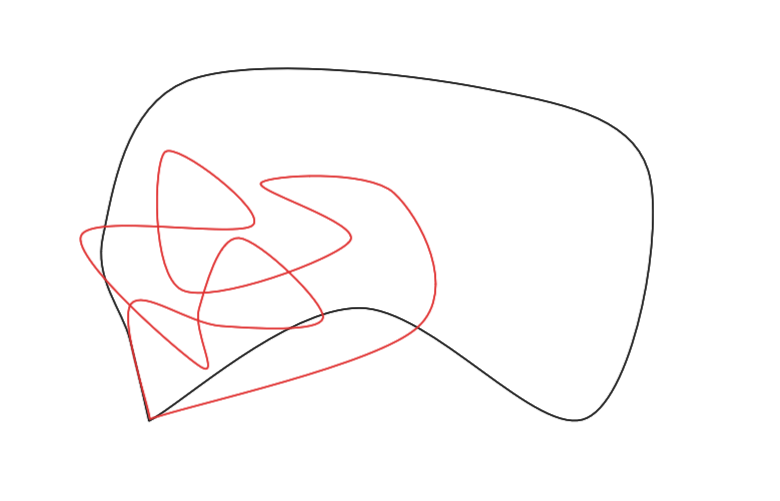
\includegraphics[width=0.8\textwidth]{bilder/CoveredAreaSketch.png}
		\caption{An example sketch showing the outlines of two different tours.}
		\label{fig:coveredAreaSketch}
	\end{centering}
\end{figure}

The above figure shows the outlines of two possible tours, the black outline being more round than the red one. 
Here, the covered area of the black tour is larger than the one of the red tour, since in the calculation, all smaller areas are accounted for regarding their overlap as well as the direction of the turns (clockwise or counter clockwise).
Thus, the many overlaps of areas and the crossings of path parts reduce the covered area value.
Using this calculation, the red tour has a lower covered area, making the black one more desirable.



Tour4Me implements a solution for the \enquote{touring problem} , which is used to describe the task of finding appealing and ideally interesting roundtrips.
To achieve a relatively good solution, two factors are taken into consideration.
First is the total profit, that can be collected within the given length restriction for the tour.
Second, is an additional quality function that assures for a relatively round tour by maximizing the area that is surrounded by the created roundtrip.
Tour4Me presents a selection of four different algorithms to calculate the tour as well as some additional customization options.
The offered choices include a Greedy Selection approach, Integer Linear Programming, MinCost with \textit{Waypoints} - a shortest paths variant - and Iterative Local Search (ILS) \cite{buchin_tour4me_2022}. 

The Greedy Selection \cite{buchin_tour4me_2022, wayahdi_greedy_2021} is the simplest algorithm which only ensures that the chosen route is a roundtrip.
The result path is built by iterating over the valid edges and picking the most profitable of these until the cycle is finished or no candidate is left.
A valid edge is determined by checking whether the start- and endpoint \textit{s} can still be reached if that selected edge is picked next.


For Integer Linear Programming \cite{buchin_tour4me_2022, graver_foundations_1975}, the touring problem must be stated in an appropriate form.
To do so, a single instance can be encoded as $\mathcal{I}(G, w, \pi, B, v_0)$, containing the Graph $G$, edge costs $w$, the profit function $\pi$, the budget (length restrictions) $B$ and the starting (and end-) point $v_0$.
Given this encoding, cycles $P=(v_0,...,v_i,...,v_0)$, which are always at most of length \textit{L}, can be built.
For the current definition, a few additional variables can be introduced to encode whether or not an edge is part of a solution (and how many times this edge occurs), whether or not an edge is the k-th edge of the solution and whether or not a vertex is the k-th vertex of a solution. 
Using these variables, constraints can be built to describe the desired behavior of the algorithm.

The MinCost algorithm \cite{buchin_tour4me_2022, gemsa_efficient_2013} needs the \textit{waypoints}, which are intermediate points used to calculate shortest paths between them (see \ref{subsubsec:runningRoutes} for more details).
These waypoints are needed because the algorithm used for the MinCost calculation is typically meant to solve shortest path problems. 
Thus, the underlying calculations would always result in not leaving the starting position without the added waypoints. 
Even though this algorithm is not originally meant to solve roundtrip problems, the implementation takes into account the cost and profits of edges to create a solution tour, which makes this method more suited to the task than simple greedy search.
To create an optimized tour, the inefficiency of paths has to be measured. 
This is done by calculating the quotient of the edge costs and the profit the edge yields. 
Using this inefficiency, a ring of candidate points $R_s$ surrounding the start-point \textit{s} can be calculated.
All points that are part of this ring have a shortest path distance of at most $\pi$.
From these, new rings $R_r$ with the same requirements can be calculated. 
The solution path is then obtained through intersecting the sets of all circles and selecting all those that intersect with $R_s$.
To ensure that the highest profit tour is returned, all possible combinations are calculated and the best of these solutions will be returned \cite{buchin_tour4me_2022}. 
Further details can be found in the original paper \cite{gemsa_efficient_2013}, which offers a Greedy Faces approach as well as two variants for the Partial Shortest Paths algorithm, of which the 2-via-routes option was implemented in Tour4Me.

Building from this solution, Iterative Local Search \cite{buchin_tour4me_2022, lu_arc_2015, verbeeck_extension_2014} can be applied to improve the found tours.
ILS is split into two main phases: the removal step and the improvement step.
The algorithm starts with a full roundtrip and then removes partial paths $P$ from the current best solution $S$ (the removal step).
After that, the previous tour now has a gap, which has to be closed by iteratively adding new vertices and edges that improve the solution profit while always staying within the given budget (the improvement step).
When adding new edges to the solution that close the path, both the profit as well as the length that these paths have must be considered. 
Since the roundtrip has a given maximum length, the profit has to be maximized while keeping track of and never exceeding this length constraint.
The best solution is improved constantly until the user selected time limit is reached \cite{buchin_tour4me_2022}.

Searching for viable edges is performed using a depth first approach, thus bounding the maximum depth of this step can drastically speed up the algorithm.
This speed up then results in more iterations of removal and improvement being possible within the given time limit.



\subsection{Roundtrip paths}
\label{subsec:Roudtrip}
There are a few tools and some research that deal with the construction of roundtrips.
Some of the papers specifically focus on running routes or tours tailored pointedly to cycling.
RouteLoops and RouteYou are two commercial tools that offer an interface to calculate tours, but don't have many customization options.
However, neither has there been much research on roundtrip generation, nor are there any tools that offer customizability.
Aside from these few approaches for roundtrip calculation, some ideas to improve the experience and training effect of running, how to assist various different sports with technology and even approaches on how to determine pleasant surroundings of paths have been developed, but these approaches have not been combined into a single application yet.



\subsubsection{Computing Running Routes}
\label{subsubsec:runningRoutes}

The problem of calculating good running roundtrips is not new.
In addition to the commercial applications, there are research papers on this subject as well.
One of these papers by Gemsa et al.\ \cite{gemsa_efficient_2013} present two approaches to handle the new routing problem the authors labeled \enquote{Jogging Problem}, which is split up into two variants: 
One being the simple version, that only aims to build a cycle that contains the starting point \textit{s} and has the desired length.
The other is a more complex version, that allows for some flexibility regarding the length of the final tour during optimization, which is named \enquote{Relaxed Jogging Problem} \cite{gemsa_efficient_2013}. 
This relaxation allows to take more factors into account to also optimize for the resulting shape, the area surrounding the tour and/or the simplicity of the path. 

The second problem is chosen as the one to optimize, since the relaxation enables the addition of conditions other than just the length of a tour.
For solving this selected problem, two different ideas are proposed.
The first approach - \enquote{Greedy Faces} - is based on the idea of extending previous cycles.
The algorithm starts with a cycle containing the starting point \textit{s} that can be selected by the user. 
This roundtrip then can be extended to gradually approach the length specified by the user. 
The second algorithm is named \enquote{Partial Shortest Paths} and uses \textit{waypoints} or \textit{via-vertices}.
These are a number of new points that can be connected using shortest paths.
When the via-vertices are connected with each other and the start, they form a roundtrip.


For both algorithms, the authors measure the badness of paths, the number of edges that are shared as well as the number of turns.
The badness is used to take the additional constraints into account. 
To reduce the possibility of having a roundtrip which turns at the end and uses all paths twice - which would effectively form a simple U-Turn (turning by 180 degrees) tour - the number of shared edges has to be minimized.
The number of turns corresponds to the complexity of the tour and is measured by a percentage of doing a full U-Turn. 
Gemsa et al.\ define the point between two edges as a \textit{turn} if the angle is larger than 15 degrees or equal and less than 180 degrees.
These turns can then be used to determine the complexity of a tour:
More turns meaning a more complex tour.

The ideas presented in this paper are also used by Thomas Pajor in his dissertation \cite{pajor_algorithm_2013}, where he talks about Computation of Jogging Routes. In the last chapter, he describes the algorithms and gives details about Greedy Faces and Partial Shortest Paths as well.

%
%\paragraph{Greedy Faces}
%
%Greedy Faces is built from an already existing path by extending it.
%For this, blocks outside the given tour that are adjacent to the current path are used.
%The previous cycle then is changed so that it encloses the chosen block and thus extends the preceding route. 
%New blocks are picked until the desired length is reached.
%To ensure only blocks that correspond to faces are picked, a preprocessing phase is introduced that identifies faces of the graph.
%During this step, first, dead-ends are removed, so the resulting graph will be two-connected.
%Faces then are defined by the edges that surround them. 
%While identifying all faces, a dual graph $G^{\star} = (V^{\star},E^{\star})$ for $G = (V,E)$ is built as well.
%
%The Greedy Faces algorithm then works on the dual graph $G^{\star}$, selects a face \textit{f} from $V^{\star}$ which has a surrounding path that contains the starting point \textit{s}. 
%Then, a Breadth First Search Tree \textit{T} is built, starting at \textit{f}, until the desired length (a relaxed version $(1 + \varepsilon) L$) is exceeded.
%The resulting tour will be a simple path iff all vertices in \textit{V} without the ones in \textit{T} are connected and contain \textit{s}.
%The final jogging path can be extracted by taking the cut edges between the tree \textit{T} and the remaining vertices.
%This always forms a cycle and thus builds a roundtrip.
%
%For building a path which optimizes all constraints, the three introduced measures for badness, number of shared edges and the number of turns are used.
%The badness function is incorporated into a different force function $\varphi (f,p) = \frac{(\text{bad}(f)-0.5)l(f)}{|\vec{d}|^2} \cdot \frac{\vec{d}}{|\vec{d}|}$ which can assign positive and negative badness values to edges.
%Furthermore, the force function uses the cost of the face and a vector $\vec{d} = \vec{p} - \vec{C}(f)$ which is built from the geometric center $\vec{C}(f)$ of a face to any point $\vec{p}$. 
%This force vector can then be used to calculate the best next edge for extending the current path by maximizing $\varphi(g) cos (\measuredangle (\varphi(g), C(f) - C(P)))$, measuring the angle between the directed force vector and the geometric center point \textit{C(P)} of the path that has been built so far.
%The force vector is used in the Breadth First Search but it doesn't have to be the only criteria.
%An extension to include other measures like roundness or complexity can be created as well. \cite{gemsa_efficient_2013}
%
%
%After the tour has been created, it will be smoothed to reduce the complexity.
%This is done by building a subset (always including \textit{s}) of the nodes contained in the created path and computing shortest paths between all vertex pairs in this subset. 
%Concatenating them will then return a smoothed path.
%This approach is extended to again take badness into account as to not create a bad final path because of the smoothing step. \cite{gemsa_efficient_2013}
%
%The greedy faces algorithm does extend an initial cycle, but it has no guarantees on the length of the final returned path.
%It can deviate without constraints from the original user specification, resulting in paths that can be way too short or way too long. \cite{gemsa_efficient_2013}
%
%
%\paragraph{Partial Shortest Paths}
%
%Since Greedy Faces cannot give any guarantees, the authors pursued a second approach to calculating results that are ensured to deviate at most by a small $\varepsilon$.
%The partial shortest paths are based on a set of via-vertices and named by the number of intermediate points created. 
%In the paper, 2-via-routes and 3-via-routes are presented.
%
%For two intermediate points, three shortest paths have to be calculated.
%These furthermore have to have a length of $\frac{1}{3} L \pm \varepsilon$, building a triangle.
%Again, the shortest path calculation used will also consider the badness of the edges when selecting them.
%Optimizing this metric will return a set of feasible candidate paths that are \enquote{nice} - as the authors describe this property - and create a ring around the starting point.
%
%From this point, another ring with a diameter of $\frac{1}{3} L \pm \varepsilon$ is calculated from every vertex within the first ring.
%All elements that are within the intersection of both rings are valid candidates for the third point to be selected. 
%The final path is created by picking the tour with a minimal badness from all feasible combinations of \textit{s} and the two other selected vertices. \cite{gemsa_efficient_2013}
%
%The three point variant 3-via-routes is an extension to improve the smoothness around the two selected vertices for building the initial triangle. 
%The algorithm then builds the ring around the starting point as in the first version but with a narrower radius of $\frac{1}{4} L \pm \varepsilon$.
%Then, an even narrower ring is created, using a new parameter $\alpha \in [0.5,1]$ as a condition for the radius of the new ring: $\frac{\alpha}{3} L \pm \varepsilon$.
%The value of $\alpha$ and a new point \textit{m} in the middle of the created path control the smoothness around the two other vertices.
%
%From the two triangle points \textit{u} and \textit{v}, new points \textit{u'} and \textit{v'} within the narrower ring are obtained by following the shortest path trees. 
%Then, new rings around these vertices are calculated, using a radius of  $\frac{2-\alpha}{4} L \pm \varepsilon$ to ensure a distance of  $\frac{1}{2} L \pm \varepsilon$ for all vertices within each of these rings.
%This results in a ring containing possible middle vertices.
%Then, for all pairs \textit{u'} and \textit{v'}, the intersection of their respective rings can be built and all middle vertices that will yield a smooth path for the two triangle points \textit{u} and \textit{v} will be selected as middle point candidates.
%Finally, the path along the vertices that has minimum badness will be returned as the result. \cite{gemsa_efficient_2013, pajor_algorithm_2013}
%
%Both, the Greedy Faces as well as the Partial Shortest Paths offer a solution to the roundtrip problem.
%They also allow for customization of the tour using different constraints. 
%This is why the Partial Shortest Paths approach is already used as one available option in Tour4Me. 
%The constraints and parameters that can be used to influence properties of the tour offer fewer customization options than it is planned for this thesis. \# TODO do I have to specify what is different from my approach for every paper I mention here?


\subsubsection{Computing Cycling Routes}
\label{subsubsec:cyclingRoutes}

For running, there are some papers discussing ideas for generating cycling tours.
Ehrgott et al.\ \cite{ehrgott_bi-objective_2012}  discuss a bi-objective model that takes travel time and \enquote{suitability for cycling} into account.
Suitability is defined as a combined measure of objective factors containing but not limited to the volume and speed of traffic on the roads, which can impact the safety of these path segments. 
However, subjective values like the individual fitness level are not taken into account for this implementation.
All objective values that are considered significant for the \textit{suitability} of the tour are accumulated into the one measure, so that there are only two values to optimize at the same time. 

The authors offer a solution for the issue that many of the values can have a different level of importance for different people. 
While some people might not want hilly routes at all, others could enjoy the challenge a certain steepness proposes. 
Because of this difference in basic preferences, Ehrgott et al.\ chose to offer a choice set of several alternative routes, from which the user can pick the one that works best for their preferences. 

This approach takes several different factors into account, but does not offer any means to influence the importance specific factors have on the generated routes beforehand.
Furthermore, the presented ideas are focused on shortest path applications, not on roundtrips.

Verbeeck et al.\ \cite{verbeeck_extension_2014} concentrate on cycle trips in their paper, which also builds a foundation for the algorithm used in Tour4Me (see \ref{subsec:Tour4Me}). 
They build a \enquote{cycle trip planning problem (CTPP)} as an alternative version of the arc orienteering problem (see section \ref{sec:aop} for further details). 
The initial idea is to use a meta-heuristic approach of ILS to build roundtrips that optimize the profit of the trip.
Since the arc orienteering problem is already NP-hard and the CTPP has an even higher complexity, attempting to solve it with an analytic, exact algorithm will not be feasible in terms of time constraints. 
Because of this complexity, the authors developed two approaches - a branch-and-cut algorithm and a meta-heuristic method - to try and solve their CTPP quickly. 
The branch-and-cut approach turned out to return results on smaller sets within a reasonable time.
However, the algorithm will be too slow for larger problem space instances.

Therefore, Vereeck et al.\ developed the ILS approach which can be split up into three phases:
The initialization, the improvement and the selection.
During the initialization the implemented algorithm gathers a first set of possible solutions by using the insert move that aims to find a path with the highest score.
The insertion starts with every arc that leaves the starting point and builds a maximum-profit path until a feasible solution is obtained.
This step is done for all possible starting points, so several solutions are created.
Then, the results from the previous step are optimized in the improvement phase. 
To do so, a part of the solution is removed during every iteration.
Next, the newly constructed gap - between the two nodes where path was removed - is closed using the same insert move from the initialization, thus improving the previous solution.
This then iterates over the whole tour until the removal encounters the end vertex (which is equivalent to the start vertex) again.

Using this approach, the authors were able to create a path within the given time constraints, build a roundtrip, ensure that it's length lies between a maximum and minimum value and optimize it's profit.
They also stated that their ideas can be used as \enquote{building blocks}  \cite{verbeeck_extension_2014} for further development.
Something Verbeeck et al.\ stress, is the fact that vertices can be visited multiple times (except the start vertex), however arcs and (if existent) their complements cannot. 
Thus they enforce trips to not take the same paths twice.

They did several benchmark tests for their implementations, but the code is not available.
Furthermore, there does not seem to be any way to try the existing implementation out and assess how many parameters are used, which of them can be changed and how much customization is possible.
The fact that the authors do not allow passing an arc twice also limits the options to select a preferred tour shape that might include those that simply run one way and have a U-Turn at the end. 


\subsubsection{RouteLoops \& RouteYou}
\label{subsubsec:routeLoopsrouteYou}

RouteLoops and RouteYou are two commercial programs that can be found and used online. 
However, neither the code itself nor information about the implementation can be accessed.

RouteLoops has two text fields for entering the starting point and the length of the trip.
Aside from that, no customization is possible.
The interface has a few features to show more information about the route.
After the calculation, distance markers or elevation can be displayed.
However, these outputs can not be used as inputs to get a route with - for example - as little elevation as possible.
The page claims that the difficulty of a route can be shown for tours that are placed within the United States.
However even when creating a route in the United States, the difficulty was not shown. 
RouteLoops also does not actually create loops but rather picks a route that has a high value (for example with a river in a park) and lets the user run along that path, turn around at the end and run back the same way.

To create a roundtrip, some waypoints are created. 
These points can be removed or more can be added in when editing the tour.
Between the waypoints, a shortest path is created to connect them. 

RouteYou offers several different user input options that will return varying results, however, picking the same option again will also give different results every time.   
Here, the roundtrips are more round than with RouteLoops, but again, elevation or difficulty are not taken into account. 
Even though both do offer the possibility to edit the returned roundtrip, this editing changes the length of the route arbitrarily.
Furthermore, the user can not specify directly what type of ground, surroundings, etc. are preferred. 




\subsection{Other running related research}
\label{subsec:otherRunningResearch}

Aside from the few directly related papers and applications, some general research regarding running with technology has been done.
Jensen and Mueller \cite{jensen_running_2014} focus on the utilization of interactive technologies that can be used to monitor or enhance the performance of athletes.
They are especially interested in how to improve these gadgets and apps to make them more usable. 
In their paper, they discuss the current state of different technologies and propose the following three questions as ideas of what aspects to focus on for further improvement:
\enquote{How to interact}, which focuses mainly on the question how interaction with any app or gadget can be designed so it won't hinder the actual activity of running;
\enquote{What information}, aiming at improving the types of information that are presented to the user while running (for example to change the running style mid run);
and \enquote{When to assist}, which addresses the timing aspect of any kind of assistance during a workout. 
They strive to find suggestions on what to focus on when trying to produce apps or gear for runners.



\subsection{Apps that assist with sports}
\label{subsec:runningApps}

Aside from Tour4Me, RouteLoops and RouteYou, another prototype for running route recommendations has been developed.
Other papers like one by Loepp and Ziegler \cite{loepp_recommending_2018} used the Partial Shortest Paths algorithm from the idea Gemsa et al.\ presented \cite{gemsa_efficient_2013} to build a recommendation based app.
However, they tried to incorporate more criteria, for example elevation levels or information about the surroundings, allowing users to pick from a variety of options when generating personalized tours. 
Furthermore, the authors added a feature to use routes of other users, but their following survey revealed that none of their users were interested in that particular feature.

The customized tours that could be generated were received well, perceived as having high quality and the difficulty was seen as low by the users.
This app is only a prototype and was never fully expanded into a full fledged product.
Currently, it runs only on smartphones that use Android. 

In the corresponding paper \cite{loepp_recommending_2018}, Loepp and Ziegler also express several issues with and shortcomings of existing apps.
Some of these problems have already been identified in the introduction of the two websites RouteLoops and RouteYou (see \ref{subsubsec:routeLoopsrouteYou}).
They also stress, that most research either concentrates on shortest paths or on the assistance with the training itself rather than finding a good route.

Apps like \textit{Runtastic}\footnote{\url{https://www.runtastic.com/}}, \textit{Sportractive}\footnote{\url{http://sportractive.com/}} or \textit{Strava}\footnote{\url{https://www.strava.com}} are designed to help runners track the tours they already ran. 
These apps measure pace, position, height meters and several other stats during a run to then be able to produce feedback for the user. 
Planning a route is not one of the features these apps offer.
And even apps that are meant to assist with the training and which create a plan like \textit{Trainingpeaks}\footnote{\url{https://www.trainingpeaks.com/}} or \textit{SportTracks}\footnote{\url{https://sporttracks.mobi/}} do not offer a feature to create routes or roundtrips with a set of preferences \cite{loepp_recommending_2018}.

A German app that is meant to provide suitable routes for a variety of different outdoor sports - \textit{Komoot}\footnote{\url{https://www.komoot.de/}} - does offer a route selection. 
However, only tours other users have planned and added can be selected. 
No customization or automated route creation is offered here. 
As Loepp and Ziegler pointed out in their user study \cite{loepp_recommending_2018}, user feedback, their preferences and the option to customize were very important features for a route generation app. 
The fact that no participant of their study decided to try out a route another member had recorded further stresses the importance of personalized route generation.


\subsection{Other tour optimization ideas}
\label{subsec:otherTourOptimization}

Aside from approaches to calculate good roundtrips and the various sports-assisting apps and technology, there is another point that can be related to generating desirable tours.
Some papers discuss the question of how to find scenic routes, which aspects impact how appealing a route is and how the availability of more panoramic routes can influence the decisions of users.
To gain some understanding of what is considered scenic and what features can lead users to take longer tours into account, Alivand et al.\ \cite{alivand_analyzing_2015} created a route choice model.
Their application calculated and displayed the shortest path from a source to a destination and additionally a set of routes that were longer (considering their length or the travel-time or both), but had more panoramic view along the path.
The points they used to decide what can be considered as a scenic view were gathered from a set of geo-tagged photos and from travel blogs.

From their testings, users were happy to take detours that were on average 90\% longer than the fastest tour.
This observation shows how important the view and surroundings can be when the goal is not necessarily to find a quick or short path, but also to take other subjective parameters into account.
The paper focused on touristic trips from a start to a specific destination, but their findings can easily be translated to other modes of travel, including roundtrips.



% kapitel2.tex
\section{Related Work}
\label{sec:relatedWork}


Much research has been done for shortest path algorithms and their optimization, however, for the - more complicated \cite{gemsa_efficient_2013} - problem of finding a round trip with several further conditions, not much work has been done yet.
While there are a few tools that can be used to calculate round trips, most of them only focus on cycling or create a very limited set of trips that do not satisfy the needs of most people, or both. 
Some examples for these tools are RouteLoops\footnote{\url{https://www.routeloops.com/}, last accessed: 22.03.2024} and RouteYou \footnote{\url{https://www.routeyou.com}, last accessed: 22.03.2024} which both do not allow for much customization of preferences. 

Adding new options for user inputs that enable a higher degree of customization can vastly improve the usability of a tool. 
The usefulness is not only determined by the implemented algorithms, but also by the interface, the data used, and the selection options presented to the user. 

As both RouteLoops and RouteYou are commercial programs, it was not possible to obtain any details about used algorithms, heuristics, meta-heuristics or even the language they used for programming these solutions.
All gathered information are collected from exploring the functionality of the two tools by hand and reading both the general information and the FAQ pages provided by the websites (for further reading see \ref{subsubsec:routeLoopsrouteYou}). 

\subsection{Tour4Me}
\label{subsec:Tour4Me}

The tool which this thesis will be based off, Tour4Me\footnote{http://tour4me.cs.tu-dortmund.de/} \cite{buchin_tour4me_2022}, incorporates some of the mentioned customization options in its web interface. 
It is possible to choose the favored ground type as well as make selections about preferred route types.
Furthermore, the user can also mark certain types as undesirable (rather than just keeping them neutral or marking them as preferable).
This allows for much more customization.
What the tool does not incorporate yet is the option to make selections about the preferred elevation or route complexity.
However, the tour can be optimized for a circular route when calculating and maximizing the covered area of the tour. 

%Currently, Tour4Me does not work for all starting points and or lengths selected by the user.
%It uses different approaches and some cannot calculate results.
%Sometimes, it works to allow for a longer computing time but sometimes, no route can be found at all.
%The goal is to add more options that will be able to return results for most or - optimally - all starting points, lengths and user customizations.

It implements a solution for the \glqq touring problem\grqq , which is used to describe the task of finding appealing and ideally interesting roundtrips.
To achieve an optimal solution, two factors are taken into consideration.
First is the total profit, that can be collected within the given length restriction for the tour.
Second is an additional quality function that assures for a relatively round tour by maximizing the area that is surrounded by the created roundtrip.
Tour4Me presents a selection of four different algorithms to calculate the tour as well as some additional customization options.
The offered choices include a Greedy Selection approach, Integer Linear Programming, MinCost with Waypoints - a shortest paths variant - and Iterative Local Search \cite{buchin_tour4me_2022}. 

The Greedy Selection is the simplest algorithm which only ensures that the chosen route is a roundtrip.
It builds its path by iterating over the valid edges and picking the most profitable of these until the cycle is finished or no candidate is left.
A valid edge is determined by checking whether the start- and endpoint \textit{s} can still be reached if that selected edge is picked next \cite{buchin_tour4me_2022}.


For Integer Linear Programming, the touring problem must be stated in an appropriate form.
To do so, a single instance can be encoded as $\mathcal{I}(G, w, \pi, B, v_0)$, containing the Graph $G$, edge costs $w$, the profit function $\pi$, the budget (length restrictions) $B$ and the starting (and end-) point $v_0$.
Given this encoding, cycles $P=(v_0,...,v_i,...,v_0)$, which are always at most of length L, can be built.
For the current definition, a few additional variables can be introduced to encode whether or not an edge is part of a solution (and how many times it occurs), whether or not an edge is the k-th edge of the solution and whether or not a vertex is the k-th vertex of a solution. 
Using these, constraints can be built to describe the desired behavior of the algorithm \cite{buchin_tour4me_2022}.

The MinCost algorithm needs the waypoints because it is typically meant to solve shortest path problems. 
Thus it would always choose not leaving the starting position without the added points. 
Even though this algorithm is not originally meant to solve roundtrip problems, it takes into account the cost and profits of edges to create a solution tour, which makes it more suited to the task than simple greedy search.
To create an optimized tour, the inefficiency of paths has to be measured. 
This is done by calculating the quotient of the edge costs and the profit the edge yields. 
Using this inefficiency, a ring of candidate points $R_s$ surrounding the start-point \textit{s} can be calculated.
All points that are part of this ring have a shortest path distance of at most $\pi$.
From these, new rings $R_r$ with the same requirements can be calculated. 
The solution path is then obtained through intersecting the sets of all circles and selecting all those that intersect with $R_s$.
To ensure the highest profit tour is returned, all possible combinations are calculated and the optimum is returned\cite{buchin_tour4me_2022}. 
Further details can be found in the original paper \cite{gemsa_efficient_2013}, which offers a Greedy Faces approach as well as two variants for the Partial Shortest Paths algorithm, of which the 2-via-routes option was implemented in Tour4Me.

Building from this solution, the Iterative Local Search can be applied to improve the found tours.
From the returned roundtrip, the algorithm removes partial paths $P$ from the current best solution $S$ and tries to iteratively add new parts that improve the solution profit while always staying within the given budget ($B-w(\frac{S}{P})$).
Since searching for viable edges is performed using a depth first approach, bounding the maximum depth of this step can drastically speed up the algorithm.
To keep track of the added length and profit, two variables ($l$ and $p$ respectively) are introduced.
These start with an initial value of one and are raised by a single increment for each iteration.
$p$ is reset when the starting point is reached by the removal step.
$l$ is reset when the maximum length for the solution is reached.
The best solution is improved constantly until the user selected time limit is reached \cite{buchin_tour4me_2022}.

\#TODO add more citations? --> see Tour4Me paper

\subsection{Roundtrip paths}
\label{subsec:Roudtrip}
As already stated above, existing tools leave out certain data like elevation or path types.
This impacts the quality of the created routes for users or even whole user groups. 
For example, people who prefer running with little to no elevation can end up with a route that takes them uphill through a park for half of the route.
While this still may be a good choice for other users - joggers who prefer more challenging routes or people who want to hike and enjoy ascending - this can be undesirable for beginners.
Some people could prefer running through the city over running through a park when the elevation matches their preferences better in the city.
For these users, the created route would be highly unfavorable, even though it matches other constraints for what is considered a nice roundtrip.
Therefore, it can be crucial to the usefulness of an app to give the user as many options to customize as possible. 


\subsubsection{RouteLoops \& RouteYou}
\label{subsubsec:routeLoopsrouteYou}
RouteLoops has two text fields for entering the starting point and the length of the trip.
Aside from that, no real customization is possible.
It does have a few features to show more information about the route like showing distance markers or elevation, however, these can not be used as inputs to get a route with - for example - as little elevation as possible.
Apparently it can also show route difficulty for the United States, however even when creating a route in the United States, no result was shown. 
RouteLoops also does not actually create loops but rather picks a route that has high value (for example with a river in a park) and lets the user run along that path, turn around at the end and run back the same way.

To crate a roundtrip, some \glqq waypoints\grqq{} are created. 
These can be removed or more can be added in when editing the tour.
Between the waypoints, it seems like a shortest path is tried 

RouteYou offers several different options that will return varying results, however, picking the same option again will also give different results every time.   
Here, the roundtrips are more round than with RouteLoops, but again, elevation or difficulty are not taken into account. 
Also, while both do offer the possibility to edit the returned roundtrip, this editing changes the length of the route arbitrarily.
Furthermore, it is not possible to specify directly what type of underground or surroundings etc. are preferred. 

\subsubsection{Computing Running Routes}
\label{subsubsec:runningRoutes}

The problem of calculating good running roundtrips is not new.
In addition to the commercial applications, there also are research papers on this subject.
One of these papers is \glqq Efficient Computation of Jogging Routes\grqq \cite{gemsa_efficient_2013} which presents two ideas to handle the new routing problem the authors labeled \glqq Jogging Problem\grqq .
It is split up into two variants: 
One being the simple version, that only aims to build a cycle that contains the starting point \textit{s} and has the desired length.
The other is a more complex version, that allows for some flexibility regarding the length of the final tour during optimization. 
Hence, it is named \glqq Relaxed Jogging Problem\grqq . 
This relaxation allows to take more factors into account to also optimize for the resulting shape, the area surrounding the tour and/or the simplicity of the path \cite{gemsa_efficient_2013}. 

The second problem is chosen as the one to optimize, since it enables the addition of other conditions than just the length of a tour.
For this, two different ideas are proposed.
The first approach - \glqq Greedy Faces\grqq - is based on the idea of extending previous cycles.
It starts with a cycle containing the starting point \textit{s} that can be selected by the user. 
This roundtrip then can be extended to gradually approach the user specified length. 
The second algorithm was named \glqq Partial Shortest Paths\grqq{} and uses via-vertices.
These are a number of new points that can be connected with shortest paths.
When the via-vertices are connected with each other and the start, they form a roundtrip \cite{gemsa_efficient_2013}.


For both algorithms, the authors measure the badness of paths, the number of edges that are shared as well as the number of turns.
The badness is used to take the additional constraints into account. 
To reduce the possibility of having a roundtrip which turns at the end and uses all paths twice - which would effectively form a simple U-Turn tour - the number of shared edges has to be minimized.
The number of turns corresponds to the complexity of the tour and is measured by a percentage of doing a full U-Turn (turning by 180 degrees). 
They define the angle between two edges as a \textit{turn} if it is larger than 15 degrees (and equal to or less than 180 degrees).
These turns can then be used to determine the complexity of a tour:
More turns meaning a more complex tour \cite{gemsa_efficient_2013}.

The ideas presented in this paper are also used by Thomas Pajor in his dissertation \glqq Algorithm Engineeering for Realistic Journey Planning in Transportation Networks\grqq \cite{pajor_algorithm_2013}, where he talks about Computation of Jogging Routes. In his last chapter, he describes details about the algorithms and mainly focusses on Greedy Faces and Partial Shortest Paths as well.

\# TODO is this too detailed with the following paragraphs? Should I shorten this by removing greedy faces and partial shortest paths?


\paragraph{Greedy Faces}

Greedy Faces is built from an already existing path by extending it.
For this, blocks outside the given tour that are adjacent to the current path are used.
The previous cycle then is changed so that it encloses the chosen block and thus extends the preceding route. 
New blocks are picked until the desired length is reached.
To ensure only blocks that correspond to faces are picked, a preprocessing phase is introduced that identifies faces of the graph.
During this step, first, dead-ends are removed, so the resulting graph will be two-connected.
Faces then are defined by the edges that surround them. 
While identifying all faces, a dual graph $G^{\star} = (V^{\star},E^{\star})$ for $G = (V,E)$ is built as well.

The Greedy Faces algorithm then works on the dual graph $G^{\star}$, selects a face \textit{f} from $V^{\star}$ which has a surrounding path that contains the starting point \textit{s}. 
Then, a Breadth First Search Tree \textit{T} is built, starting at \textit{f}, until the desired length (a relaxed version $(1 + \varepsilon) L$) is exceeded.
The resulting tour will be a simple path iff all vertices in \textit{V} without the ones in \textit{T} are connected and contain \textit{s}.
The final jogging path can be extracted by taking the cut edges between the tree \textit{T} and the remaining vertices.
This always forms a cycle and thus builds a roundtrip.

For building a path which optimizes all constraints, the three introduced measures for badness, number of shared edges and the number of turns are used.
The badness function is incorporated into a different force function $\varphi (f,p) = \frac{(\text{bad}(f)-0.5)l(f)}{|\vec{d}|^2} \cdot \frac{\vec{d}}{|\vec{d}|}$ which can assign positive and negative badness values to edges.
Furthermore, the force function uses the cost of the face and a vector $\vec{d} = \vec{p} - \vec{C}(f)$ which is built from the geometric center $\vec{C}(f)$ of a face to any point $\vec{p}$. 
This force vector can then be used to calculate the best next edge for extending the current path by maximizing $\varphi(g) cos (\measuredangle (\varphi(g), C(f) - C(P)))$, measuring the angle between the directed force vector and the geometric center point \textit{C(P)} of the path that has been built so far.
The force vector is used in the Breadth First Search but it doesn't have to be the only criteria.
An extension to include other measures like roundness or complexity can be created as well. \cite{gemsa_efficient_2013}
 

After the tour has been created, it will be smoothed to reduce the complexity.
This is done by building a subset (always including \textit{s}) of the nodes contained in the created path and computing shortest paths between all vertex pairs in this subset. 
Concatenating them will then return a smoothed path.
This approach is extended to again take badness into account as to not create a bad final path because of the smoothing step. \cite{gemsa_efficient_2013}

The greedy faces algorithm does extend an initial cycle, but it has no guarantees on the length of the final returned path.
It can deviate without constraints from the original user specification, resulting in paths that can be way too short or way too long. \cite{gemsa_efficient_2013}


\paragraph{Partial Shortest Paths}

Since Greedy Faces cannot give any guarantees, the authors pursued a second approach to calculating results that are ensured to deviate at most by a small $\varepsilon$.
The partial shortest paths are based on a set of via-vertices and named by the number of intermediate points created. 
In the paper, 2-via-routes and 3-via-routes are presented.

For two intermediate points, three shortest paths have to be calculated.
These furthermore have to have a length of $\frac{1}{3} L \pm \varepsilon$, building a triangle.
Again, the shortest path calculation used will also consider the badness of the edges when selecting them.
Optimizing this metric will return a set of feasible candidate paths that are \glqq nice\grqq{} - as the authors describe this property - and create a ring around the starting point.

From this point, another ring with a diameter of $\frac{1}{3} L \pm \varepsilon$ is calculated from every vertex within the first ring.
All elements that are within the intersection of both rings are valid candidates for the third point to be selected. 
The final path is created by picking the tour with a minimal badness from all feasible combinations of \textit{s} and the two other selected vertices. \cite{gemsa_efficient_2013}

The three point variant 3-via-routes is an extension to improve the smoothness around the two selected vertices for building the initial triangle. 
The algorithm then builds the ring around the starting point as in the first version but with a narrower radius of $\frac{1}{4} L \pm \varepsilon$.
Then, an even narrower ring is created, using a new parameter $\alpha \in [0.5,1]$ as a condition for the radius of the new ring: $\frac{\alpha}{3} L \pm \varepsilon$.
The value of $\alpha$ and a new point \textit{m} in the middle of the created path control the smoothness around the two other vertices.

From the two triangle points \textit{u} and \textit{v}, new points \textit{u'} and \textit{v'} within the narrower ring are obtained by following the shortest path trees. 
Then, new rings around these vertices are calculated, using a radius of  $\frac{2-\alpha}{4} L \pm \varepsilon$ to ensure a distance of  $\frac{1}{2} L \pm \varepsilon$ for all vertices within each of these rings.
This results in a ring containing possible middle vertices.
Then, for all pairs \textit{u'} and \textit{v'}, the intersection of their respective rings can be built and all middle vertices that will yield a smooth path for the two triangle points \textit{u} and \textit{v} will be selected as middle point candidates.
Finally, the path along the vertices that has minimum badness will be returned as the result. \cite{gemsa_efficient_2013, pajor_algorithm_2013}

Both, the Greedy Faces as well as the Partial Shortest Paths offer a solution to the roundtrip problem.
They also allow for customization of the tour using different constraints. 
This is why the Partial Shortest Paths approach is already used as one available option in Tour4Me. 
The constraints and parameters that can be used to influence properties of the tour offer fewer customization options than it is planned for this thesis. \# TODO do I have to specify what is different from my approach for every paper I mention here?


\paragraph{Computational Complexity}

Aside from introducing two methods to calculate roundtrip tours for running, this paper also presents a proof for the computational complexity of their Simple and Relaxed Jogging Problems.
The authors show NP hardness by reduction of Hamiltonian Cycle to the optimization problem corresponding to their original problems.\cite{gemsa_efficient_2013}

 \# TODO add the actual proof?


\paragraph{Other running related research}
Aside from the few concretely related papers and applications, some general research regarding running with technology has been done.
Jensen and Mueller focus on the usage of interactive technologies that can be used to monitor or enhance the performance of athletes.
They are especially interested in how to improve these gadgets and apps to make them more usable. 
In their paper, they discuss the current state of different technologies and propose the following three questions as ideas on what aspects to focus for further improvement:
\glqq How to interact\grqq , which focuses mainly on the question how interaction with any app or gadget can be designed so it won't hinder the actual activity of running.
\glqq What information \grqq , aiming at improving the types of information that are presented to the user while running (for example to change the running style mid run).
And \glqq When to assist\grqq , which addresses the timing aspect of any kind of assistance during a workout. 
They strive to find suggestions on what to focus when trying to produce apps or gear for runners.

Other papers like \cite{loepp_recommending_nodate} by Loepp and Ziegler used the Partial Shortest Paths algorithm from \cite{gemsa_efficient_2013} to build a recommendation based app.
However, they tried to incorporate more criteria, for example elevation or surroundings, allowing users to pick from a variety of options when generating personalized tours. 
Furthermore, the authors added a feature to use routes of other users, but their following survey revealed that no user was interested in that particular feature.
The customized tours that could be generated were received well, perceived as having high quality and the difficulty was seen as low by the users.
This app is only a prototype and was never fully expanded into a full fledged product.
Currently, it runs on Android smartphones only. 







\subsubsection{Computing Cycling Routes}
\label{subsubsec:cyclingRoutes}
As for running, there are some papers discussing ideas for generating cycling tours.
Ehrgott et al. discuss a bi-objective model that takes travel time and \glqq suitability for cycling\grqq{} into account.
This suitability is defined as a combined measure of objective factors. 
These contain for example the volume and speed of traffic on the roads, which can impact the safety of these path segments. 
But elevation and steepness of the terrain and similar values are taken into account.
They all are accumulated into the one measure of suitability, so that there are only two values to optimize at the same time. \cite{ehrgott_bi-objective_2012} 

The authors do offer a solution for the fact that many of the values can have a different importance for every person. 
While some people might not want hilly routes at all, others could enjoy the challenge they propose. 
Because of this, they chose to offer a choice set of several alternative routes, from which the user can pick the one that works best for their preferences. \cite{ehrgott_bi-objective_2012}

This approach does take several different factors into account, but does not offer any means to influence their importance on the generated routes beforehand.
Furthermore, the presented ideas are focused on shortest path applications, not on roundtrips.

Verbeeck et al. do concentrate on cycle trips in their paper. 
They build a \glqq cycle trip planning problem (CTPP)\grqq{} as a different version of the arc orienteering problem. 
The initial idea is to use a meta-heuristic approach of Iterated Local Search (ILS) to build roundtrips that optimize the profit of the trip.
Since the arc orienteering problem is already NP-hard and the CTPP is even more complex, attempting to solve it with an analytic, exact algorithm will not be feasible in terms of time constraints. 
Because of this, the authors developed two approaches - a branch-and-cut algorithm and a meta-heuristic method - to try and solve their CTPP quickly. 
The branch-and-cut approach turned out to return results on smaller sets, but will be too slow for larger problem space instances. \cite{verbeeck_extension_2014}

Therefore, they developed the ILS approach which can be split up into three phases:
The initialization, the improvement and the selection.
During the initialization gathers a first set of possible solutions by using the insert move that aims to find a path with the highest score.
It starts with every arc that leaves the starting point and builds a maximum-profit path until it obtains a feasible solution.
This step is done for all possible starting points, so several solutions are created.
These are then optimized in the improvement phase. 
To do so, a part of the solution is removed during every iteration.
Then the newly constructed gap - between the two nodes where path was removed - is closed using the same insert move from the initialization, thus improving the previous solution.
This then iterates over the whole tour until the removal encounters the end vertex (which is equivalent to the start vertex) again. \cite{verbeeck_extension_2014}

Using this approach, the authors can create a path within the given time constraints, build a roundtrip, ensure that it's length lies between a maximum and minimum value and optimize it's profit.
They also stated that their ideas can be used as \glqq building blocks\grqq{} for further development.
A thing they stress is the fact that vertices can be visited multiple times (except the start vertex), however arcs and (if existent) their complements cannot. 
Thus they enforce trips to not take the same paths twice. \cite{verbeeck_extension_2014}

They did several benchmark tests for their implementations, but the code is not available.
Furthermore, there does not seem to be any way to try out the existing implementation and assess how many parameters are used, which of them can be changed and how much customization is possible.
The fact that the authors do not allow passing an arc twice also limits the options to select a preferred tour shape that might include those that simply run one way and have a U-Turn at the end. 



\subsection{Apps that assist with sports}
\label{subsec:runningApps}

Aside from Tour4Me, RouteLoops and RouteYou, another prototype for running route recommendations has been developed.
In the corresponding paper\cite{loepp_recommending_nodate}, the authors express the problems with existing apps, some of which have already been identified in the introduction of the two websites (see \ref{subsubsec:routeLoopsrouteYou}).
They also stress, that most research either concentrates on shortest paths or - if it is research and app development specifically for running - on the assistance with the training itself rather than finding a good route.
Apps like \textit{Runtastic}\footnote{\url{https://www.runtastic.com/}}, \textit{Sportractive}\footnote{\url{http://sportractive.com/}} or \textit{Strava}\footnote{\url{https://www.strava.com}} are designed to help runners track the tours they already ran. 
They measure pace, position, height meters and several other stats to then be able to present the user feedback of the run they've done. 
Planning a route is not one of the features these apps offer.
And even apps that are meant to assist with the training and which create a plan like \textit{Trainingpeaks}\footnote{\url{https://www.trainingpeaks.com/}} or \textit{SportTracks}\footnote{\url{https://sporttracks.mobi/}} do not offer a feature to create routes or roundtrips with a set of preferences\cite{loepp_recommending_nodate}.

A German app that is meant to provide suitable routes for a variety of different outdoor sports - \textit{Komoot}\footnote{\url{https://www.komoot.de/}} - does offer a route selection. 
However, it relies only on tours other users have planned and added. No customization or route creation is offered here. 
As the authors of the paper "Recommending Running Routes: Framework and Demonstrator"\cite{loepp_recommending_nodate} pointed out in their user study, it is very important to take user preferences into account. 
No participant of the study decided to try out a route another member had recorded, which further stresses the importance of personalized route generation\cite{loepp_recommending_nodate}.

\subsection{Other tour optimization ideas}
\label{subsec:otherTourOptimization}

Aside from approaches to calculate good roundtrips and the various sports-assisting apps and technology, there is another point that can be related to generating desirable tours.
Some papers discuss the question of how to find scenic routes, what aspects impact how appealing a route is and how the availability of more panoramic routes can influence the decisions of users.
To gain some understanding of what is considered scenic and what features can lead users to take longer tours into account, the authors created a route choice model.
This showed the shortest path from a source to a destination and additionally a set of routes that were longer (considering their length or the travel-time or both), but had more scenic view along it.
These points that were considered panoramic were gathered from a set of geo-tagged photos and from travel blogs. \cite{alivand_analyzing_2015}

From their experiments, users were happy to take detours that were on average 90\% longer than the fastest tour.
This shows how important the view and surroundings can be when the goal is not only to be quick, but also takes different subjective parameters into account.
The paper focused on touristic trips from a start to a specific destination, but their findings can easily be translated to other modes of travel, including roundtrips. \cite{alivand_analyzing_2015}




% kapitel2.tex
\chapter{Fundamentals and Background}
\label{chapter:fundamentals}

As stated in the \href{chapter:introduction}{introduction}, most routing algorithms focus on shortest paths between two or more points.
Many of those have been reviewed in several different surveys \cite{madkourSurveyShortestPathAlgorithms2017, sommerShortestpathQueriesStatic2014, wayahdiGreedyAStarDijkstra2021}.
Additionally, there have been many more heuristic approaches, like local search variants \cite{braysyVehicleRoutingProblem2005, irnichSequentialSearchIts2006, ropkeHeuristicExactAlgorithms2005} or different neighborhood based ideas \cite{braysyVehicleRoutingProblem2005, irnichSequentialSearchIts2006, ropkeHeuristicExactAlgorithms2005}.
Much research has been done and is still ongoing for these kinds of problems, stemming from the fact that many routing problems (for example the traveling salesman problem (TSP) \cite{gendreauHandbookMetaheuristics2010} or the vehicle routing problem \cite{braysyVehicleRoutingProblem2005, irnichSequentialSearchIts2006}) are NP-hard \cite{reineltTravelingSalesmanComputational2003}. 
Furthermore, finding a shortest path is important in various parts of daily life.
Whether it is the best way to get to work or to a supermarket by car or bike, a good way to minimize travel time by bus or any other trip from one place to another.
Additionally, shortest paths are not limited to real-world networks but can also prove useful for social networks or any form of digital network. \cite{madkourSurveyShortestPathAlgorithms2017}

\section{Shortest Path algorithms}
\label{sec:shortestPath}

For calculating shortest path trips from one starting point s to a destination d, several different approaches can be used.
This problem has been well-studied and still continues to advance in terms of quality of the returned paths as well as in optimizing the running time of algorithms.
Thus, the number of ideas to solve it is enormous. 

Generally most shortest path problems are in one of two categories: they are either single-source shortest paths (SSSP) or all-pairs shortest paths(APSP).
The first only uses a starting point and tries to find the one shortest path between it and all other vertices.
The second aims to find shortest paths between all vertices of a graph, which can be necessary for transportation networks and similar use cases. 
Aside from these two categories, many more can be found to describe and sort types of approaches. 
Madkour et al propose a taxonomy to help classify the different algorithms into specific categories. \cite{madkourSurveyShortestPathAlgorithms2017} 

Which of these algorithms performs best is typically dependent on the type of graph it is being used on, the graph's structure and the specific problem to be solved. 
A graph can be categorized as planar or not, directed or undirected, weighted or not (and carry only non-negative weights or allow negative ones as well), they can contain cycles or be acyclic and many more. 
These different types determine which algorithms can be used as well as which will return better results.

\subsection{Single Source Shortest Paths}


\subsection{All Pairs Shortest Paths}


\subsection{Heuristic Approaches}

Additionally to exact approaches, heuristics can be used to improve the runtime of an algorithm.
A heuristic is a technique that is based on experience or statistical insights.
The downside of using such an approach is, that there will no longer be a guarantee that the result is the global optimum, as heuristics specifically only find partial or approximate solutions to a given problem. 
In many cases where it would take too much time or space to find the actual optimal solution, heuristics can be used to find the best possible solution within the given bounds.

For these, several different ideas have been formed. 
These can then be categorized into construction heuristics, improvement heuristics and meta-heuristics \cite{ropkeHeuristicExactAlgorithms2005}.
Sometimes, a fourth category for two-phase heuristics is included as well (see \cite{laporteClassicalHeuristicsCapacitated2002a}).

\#TODO is this correct for heuristics in general? The paper refers to heuristics for VRP

Construction heuristics build their solution from a starting point until a certain boundary is reached. 
They typically don't have a separate improvement phase.
Improvement heuristics try to improve an already existing solution.
They perform improvement steps several times until a specified boundary is reached.
These boundaries can be e.g. a time limit or reaching the threshold for a good enough approximation.
(Iterative) Local Search and Neighborhoods are examples of improvement heuristics that can be used to reach a more optimized solution. \cite{laporteClassicalHeuristicsCapacitated2002a, ropkeHeuristicExactAlgorithms2005}



\section{Meta-heuristics}
\label{sec:metaHeuristics}

Metaheuristics are a form of heuristic approaches.
As such, they also try to find an approximate solution to a problem that is as optimal as possible.
The distinction between classical heuristics and meta-heuristics is, that the latter are combined with additional strategies.
These are used to enable the meta-heuristics to not produce only solution that are locally optimal, but to broaden the search space they can use for finding optima.

Classical heuristics oftentimes carry the inherent risk of only finding a local optimum that can be far from the actual global one.
To reduce this risk, higher level approaches are necessary.
These can include using several neighborhood structures to broaden the search space or entirely new concepts like the Ant Colony approach or Genetic Algorithms. \cite{gendreauHandbookMetaheuristics2010}

Some of these meta-heuristic ideas that will be used in this thesis will be explained in the following subsections.



\subsection{Ant Colony}
\label{subsec:antColonyBackground}

\subsection{Genetic Algorithms}
\label{subsec:geneticAlgorithmsBackground}

\subsection{Simulated Annealing}
\label{subsec:simulatedAnnealingBackground}
% kapitel2.tex
\chapter{Implemented Changes}
\label{chapter:implementedChanges}

This work extends Tour4Me\footnote{\url{http://tour4me.cs.tu-dortmund.de/}}, which is an application written in C++ and HTML. 
The implemented interface uses C\# as programming language to enable easy porting of the web application to a desktop or mobile application.
To improve the query times, a spatial database was added. 
Reasons for and positive effects of this decision are described in the following section.

Furthermore, not only the language and data access was changed.
New options and parameters to improve the customizability of preferences for a generated tour were added as well.
These changes had to be incorporated into an upgraded front end design (see sections \ref{subsec:interfaceAndFrontendChanges} and \ref{sec:parameterChanges}) as well as into the back end and all solvers (see section \ref{sec:algorithmicChanges}). 


\section{Application}
\label{sec:application}

To include the various changes, the whole application was changed.
The Open Street Map (OSM) data are downloaded and stored in a database.
The graph for calculating the roundtrips is thus build from the new database.
Furthermore, the whole design of the front end was changed to improve the overview and general user experience as well as to allow for the addition of new customization options.
Lastly, the algorithms to choose from have been extended by two additional meta-heuristic approaches.

\subsection{New Architecture}
\label{sec:newArchitecture}

For the new application, the architecture had to be re-structured.
An illustration of the new design is shown in figure \ref{fig:architecture}.
Instead of reading the data for the graph from a static .txt file, which contains all the nodes and edges for Dortmund, a database is used to manage the nodes, edges, their additional information and the relationships between them. 
It can be filled with the data needed by using an import python script that creates an osmnx-graph\footnote{\url{https://osmnx.readthedocs.io/en/stable/}, last accessed: 15.04.2024}\footnote{\url{https://networkx.org/}, last accessed: 22.03.2024}\footnote{\url{https://wiki.openstreetmap.org}, last accessed: 22.03.2024}\footnote{\url{https://wiki.openstreetmap.org/wiki/Main_Page}, last accessed: 19.04.2024} add all references for a user specified location. 
From this graph, the nodes and edges can be extracted alongside their additional information.
For the current use case, nodes are stored with their OSM-ID, which is transformed into a UUID, their latitude and longitude coordinates as well as their elevation profile and tags of the surroundings they are placed in.
The elevation data has to be acquired from a different source than OSM, since they do not use a height profile. 
A few open source providers were available, but ultimately, Open-Elevation\footnote{\url{https://open-elevation.com/}, last accessed: 20.03.2024} was used. 

Since most open source providers have a limited bandwidth to supply users with data based on their API-calls, the opportunity to use a locally hosted version that Open-Elevation offered was very important to assure usability.
When using the python script to create and fill the database and its tables, the Open-Elevation data needs to be available.
A local docker container with the respective data can be used to access the needed information without being bound to the servers and their throughput boundaries.

The used database is Microsoft SQL Server Management Studio\footnote{\url{https://learn.microsoft.com/en-us/sql/sql-server/sql-docs-navigation-guide?view=sql-server-ver16}, last accessed: 22.03.2024}, which can handle spatial data, supports spatial queries and works well in combination with the C\# implementation.

The back end is written in C\#\footnote{\url{https://learn.microsoft.com/en-us/dotnet/csharp/}, last accessed: 22.03.2024}, as this language allows for the opportunity to also create a mobile- or desktop application in addition to the web application that already exists (see \ref{sec:futureWork}).
Furthermore, C\# allows for using SQL queries and filtering using LINQ for easy runtime database querying\footnote{\url{https://docs.telerik.com/devtools/aspnet-ajax/controls/grid/asp.net-3.5-features/linq-to-sql---binding-and-automatic-crud-operations}, last accessed: 22.03.2024}.


The front end is implemented using HTML\footnote{\url{https://devdocs.io/html/}, last accessed: 22.03.2024}, CSS\footnote{\url{https://devdocs.io/css/}, last accessed: 22.03.2024}, JavaScript\footnote{\url{https://devdocs.io/javascript/}, last accessed: 22.03.2024} and C\# code behind. 
Here, the base-styling is done using bootstrap\footnote{\url{https://getbootstrap.com/docs/4.3/getting-started/introduction/}, last accessed: 22.03.2024}, but additional custom CSS is added to create a nature-based color palette (\#TODO references to color theory stuff?) as well as several effects for the side and bottom menus.
To realize the communication between front end and back end, Ajax-queries\footnote{\url{https://api.jquery.com/category/ajax/}. last accessed: 22.03.2024} are used.

The map is a leaflet\footnote{\url{https://leafletjs.com/}, last accessed: 20.03.2024} visualization that shows Open Street Map data.
The leaflet map allows to set markers, add a search bar, create polygons - which are used to illustrate the generated routes - and offers an open source map view. 


\begin{figure}[ht]
	\hspace*{-25 pt}
	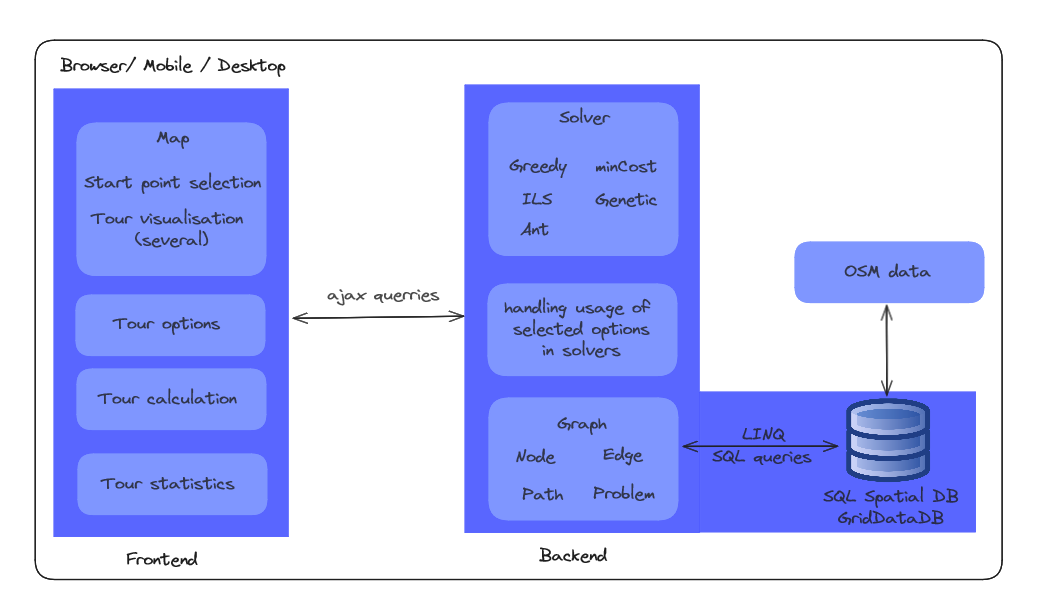
\includegraphics[width=1.1\textwidth]{bilder/Implementation Architecture.png}
	\caption{Visualization of the used architecture}
	\label{fig:architecture}
\end{figure}


In the above visualization, the whole application, the distinct parts and features are illustrated. 
The front end is realized as a web application, running in the browser but can also be customized to be executable as a mobile or desktop application (see \ref{sec:futureWork}).
Here, the map is visualized using leaflet. 
In this map, the marker can be set to the current location - if the permission to access the data is granted.
However simply searching for a specific address, drag-and-dropping the marker on the map, or scrolling the map and selecting a position by clicking on the place to mark are also possible. 
Furthermore, the visualization of the calculated tours is also realized using the map and a polygon built from the respective points.
For debug purposes, there is a feature to show the whole graph that is being used for the calculation using the current maximum length.

In addition to the main feature - the map - the front end also contains two menus:
One holding the parameters the user can use to customize the tours according to their preferences and the information menu containing a report of the core data of the calculated path that is being visualized. 
A more detailed description of the front end design, concept sketches and the final implementation are outlined in subsection \ref{subsec:interfaceAndFrontendChanges}.

\subsection{Database}
\label{subsection:database}

The database is a relational database using Microsoft SQL server, administered in Microsoft SQL Server Management Studio.
This database also allows to use spatial data, which was an important feature for storing and processing the nodes and edges.
Using the spatial features enables the possibilities to filter nodes within a given radius, retrieving only a relevant subset of data points.
This filtering option within the database significantly speeds up the data retrieval as well as the graph creation.
Compared to the previous method of generating a fixed graph for the city of Dortmund, the database offers further important advantages:
Far more nodes than only points within Dortmund can be used.
Despite the database creation and the adding of points being relatively slow, this is a process that only needs to be ran once and does not affect the tour calculation. 
Once the data has been added, all points can be accessed without needing to retrieve the whole database.

To create the database, a python script is used. \# TODO if added, describe parameters and how to use the script with them
This script first creates an osmnx graph from OSM data using the \texttt{graph\textunderscore from\textunderscore place} function
\begin{lstlisting}
	ox.graph_from_place(place_name, network_type='all', custom_filter=custom_filter)
\end{lstlisting}

Here, the \texttt{place\textunderscore name} is the name of the place for which osmnx data should be gathered.
For a city, the city's name, state and country need to be added. 
If a whole state should be selected, the state name and country are required.
The network\textunderscore type has six values to choose from\footnote{\url{https://osmnx.readthedocs.io/en/stable/user-reference.html\#module-osmnx.settings}, last accessed: 19.04.2024}: "all\textunderscore private", "all", "bike", "drive", "drive\textunderscore service", and "walk". 

The \texttt{custom\textunderscore filter} is defined to select only those edges, where walking, running and cycling is possible by specifically de-selecting respective highway types:

\begin{lstlisting}
	custom_filter = '["highway"]["highway"!~"motorway|trunk|proposed|construction|motorway_link|trunk_link"]'
\end{lstlisting}

The excluded types are used for the following street types according to the OSM Wiki:


Next, the elevation data has to be added for the nodes of this graph.
These information are not part of osmnx but need to be retrieved from a different source.
For this thesis, Open Elevation\footnote{\url{https://open-elevation.com/}, last accessed: 20.03.2024} was used.


\begin{table}[ht]
	\centering
	\begin{tabular}{l|l}
		Highway type & Description\\
		\hline
		motorway & A restricted access major divided highway, normally with 2\\ 
		& or more running lanes plus emergency hard shoulder.\\
		& Equivalent to the Freeway, Autobahn, etc..  \\
		trunk & The most important roads in a country's system that aren't \\
		& motorways. (Need not necessarily be a divided highway.) \\
		proposed & For planned roads. \\
		construction & For roads under construction. \\
		motorway\textunderscore link & The link roads (sliproads/ramps) leading\\
		& to/from a motorway from/to a motorway or lower class highway. \\
		& Normally with the same motorway restrictions. \\
		trunk\textunderscore link & The link roads (sliproads/ramps) leading \\
		& to/from a trunk road from/to a trunk road or lower class highway. 
	\end{tabular}
	\caption[OSM highway types]{This table shows a listing of different OSM highway types and their definition taken from the Wiki page\protect\footnotemark}
	\label{tab:osmHighwayTypes}
\end{table}

\footnotetext{\url{https://wiki.openstreetmap.org/wiki/Key:highway}, last accessed: 19.04.2024}
The 


\subsection{Interface and Front end changes}
\label{subsec:interfaceAndFrontendChanges}

\begin{figure}[H]
	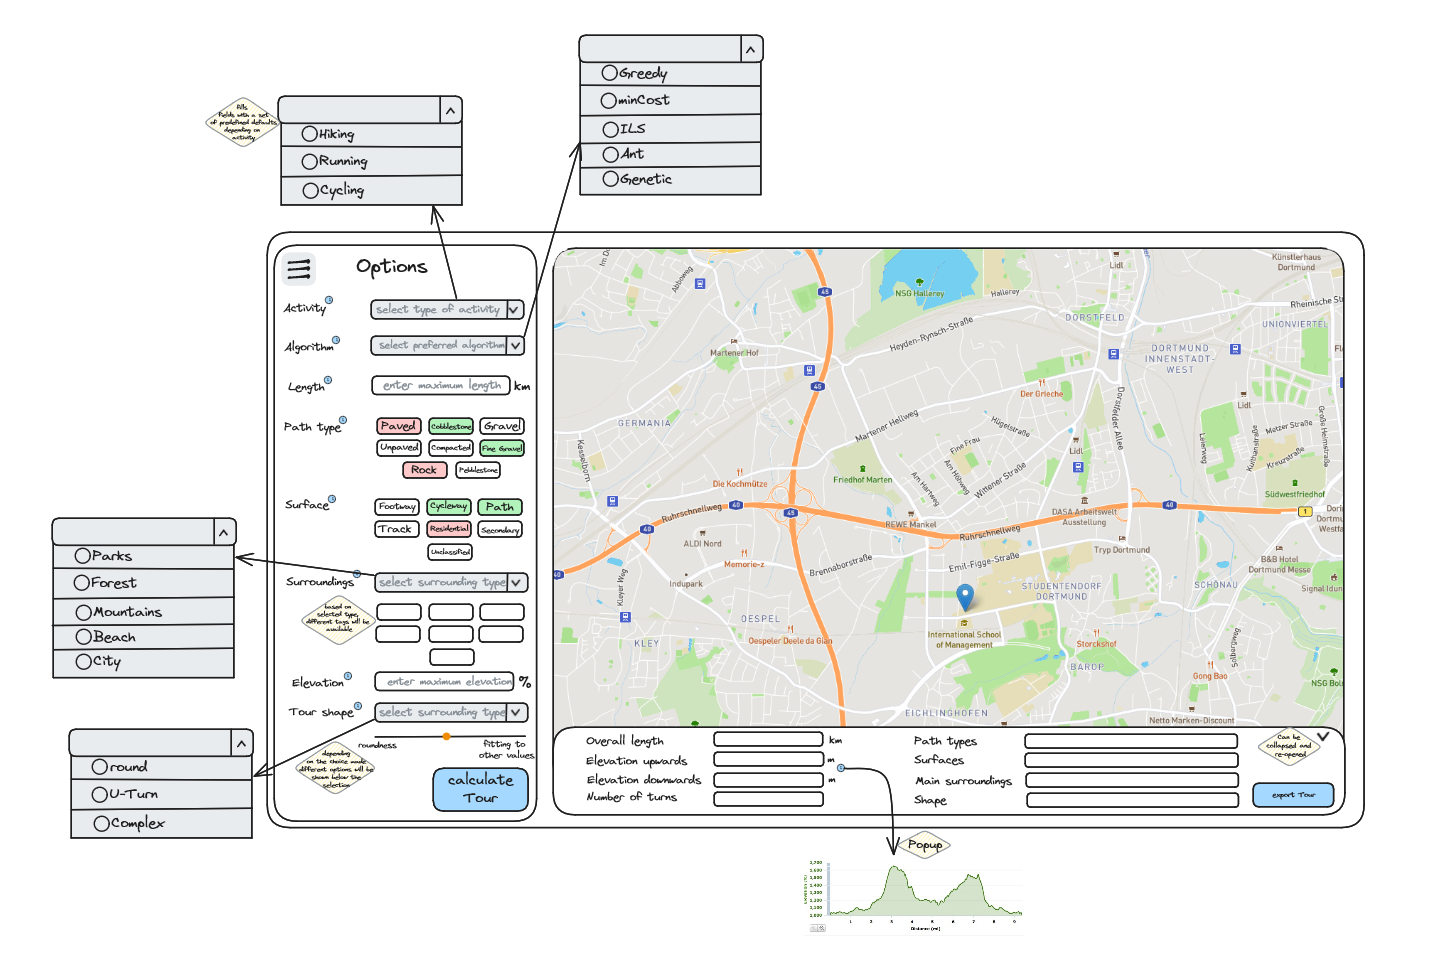
\includegraphics[width=0.9\linewidth]{bilder/Concept new Frontend design.png}
	\caption{Design concept for the front end view, including descriptions for drop-downs and pop-ups}
	\label{fig:frontendConcept}
\end{figure}


\begin{figure}[H]
	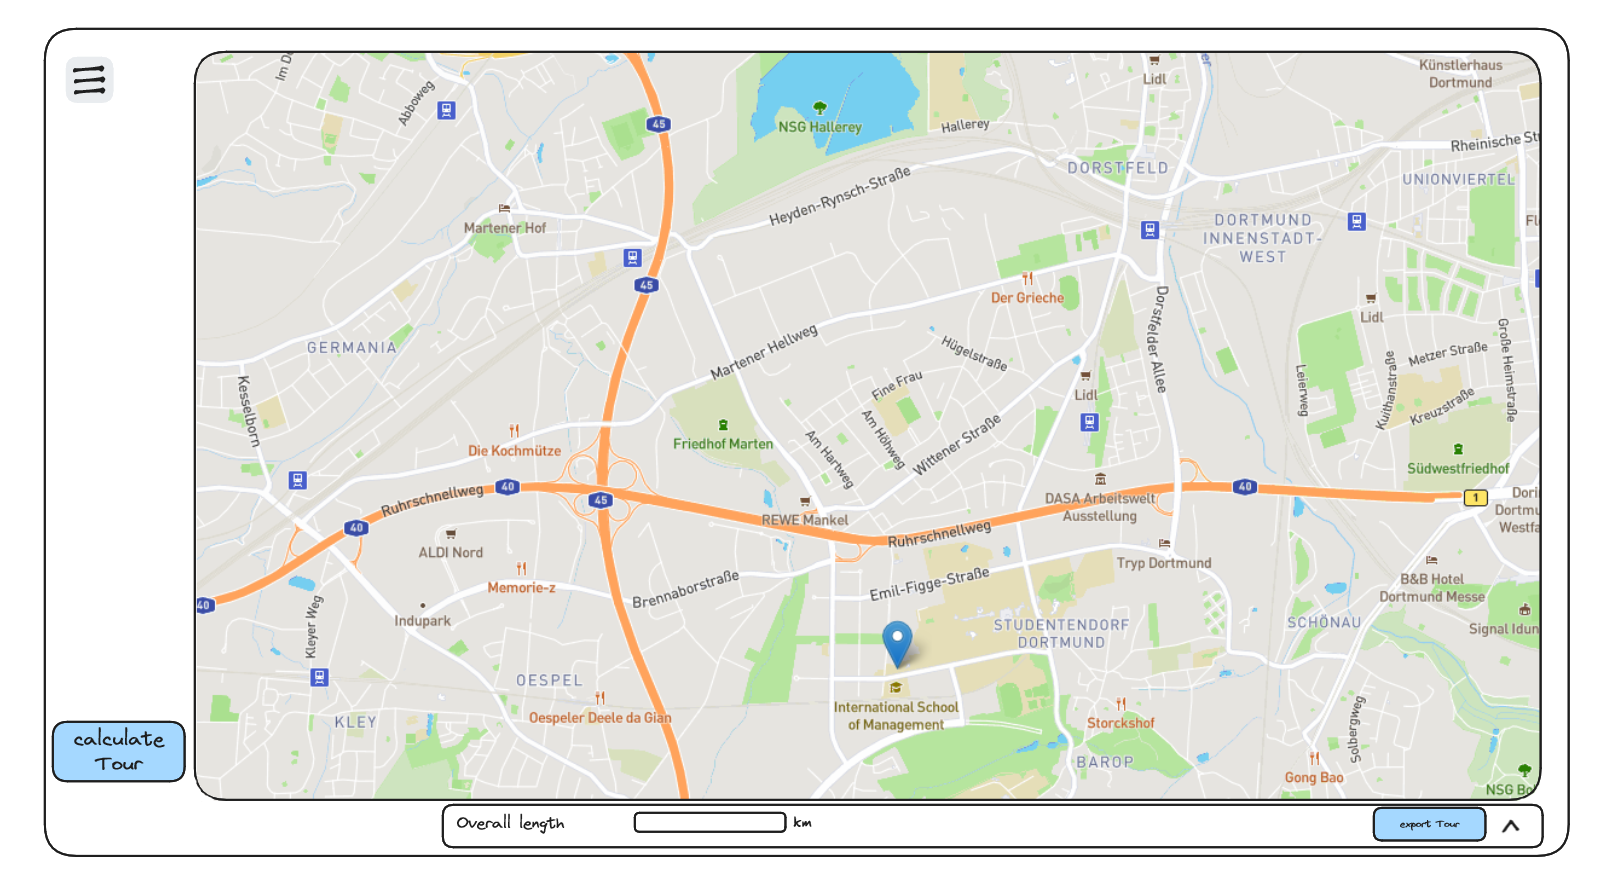
\includegraphics[width=0.9\linewidth]{bilder/Concept burger menu and stats hidden.png}
	\caption{Design concept for the front end view with all menus folded}
	\label{fig:frontendConceptMenusClosed}
\end{figure}


\begin{figure}[H]
	\begin{subfigure}[t]{0.9\linewidth}
		\centering
		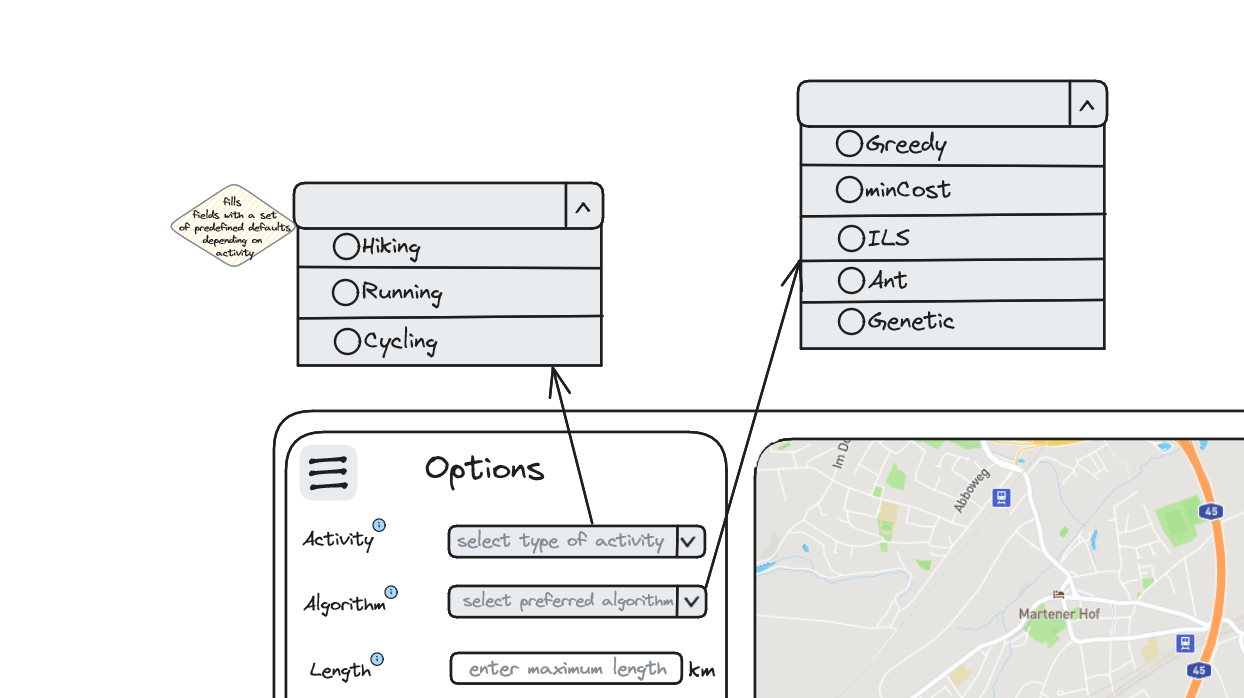
\includegraphics[width=\linewidth]{bilder/Concept closeup activity, algorithm.png}
		\caption{Design concept for the front end view, closeup of activity and algorithm dropdowns}
		\label{fig:frontendConceptCloseupDropdowns}	
	\end{subfigure}
	\hfill
	\begin{subfigure}[t]{0.9\linewidth}
		\centering
		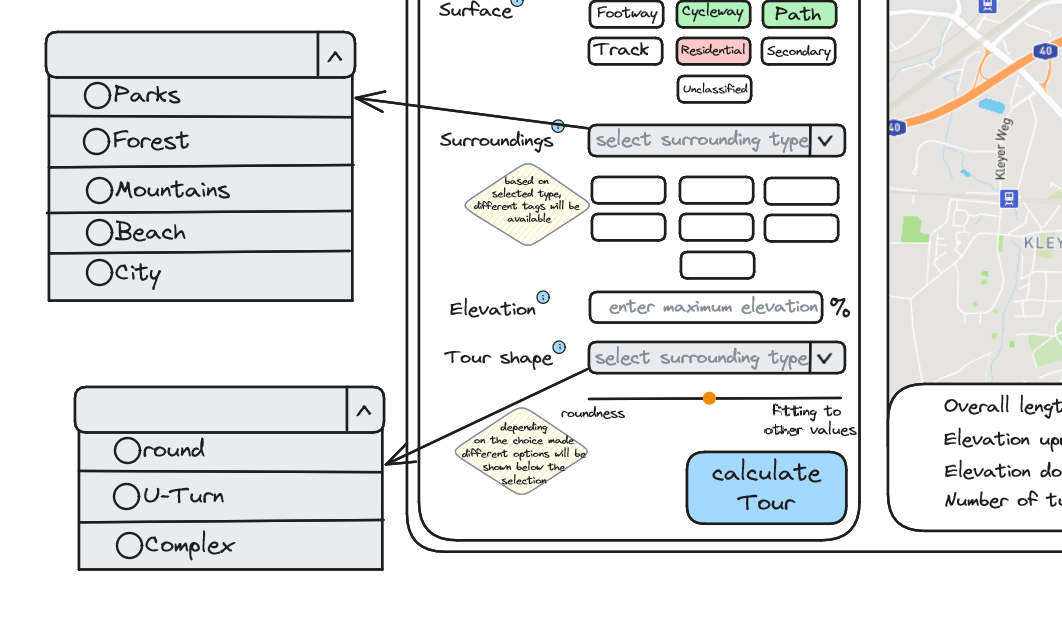
\includegraphics[width=\linewidth]{bilder/Concept closeup surroundings, tour shape.png}
		\caption{Design concept for the front end view, closeup of a surrounding and Tour shape}
		\label{fig:frontendConceptCloseupButtons}		
	\end{subfigure}
\end{figure}


\begin{figure}[H]
	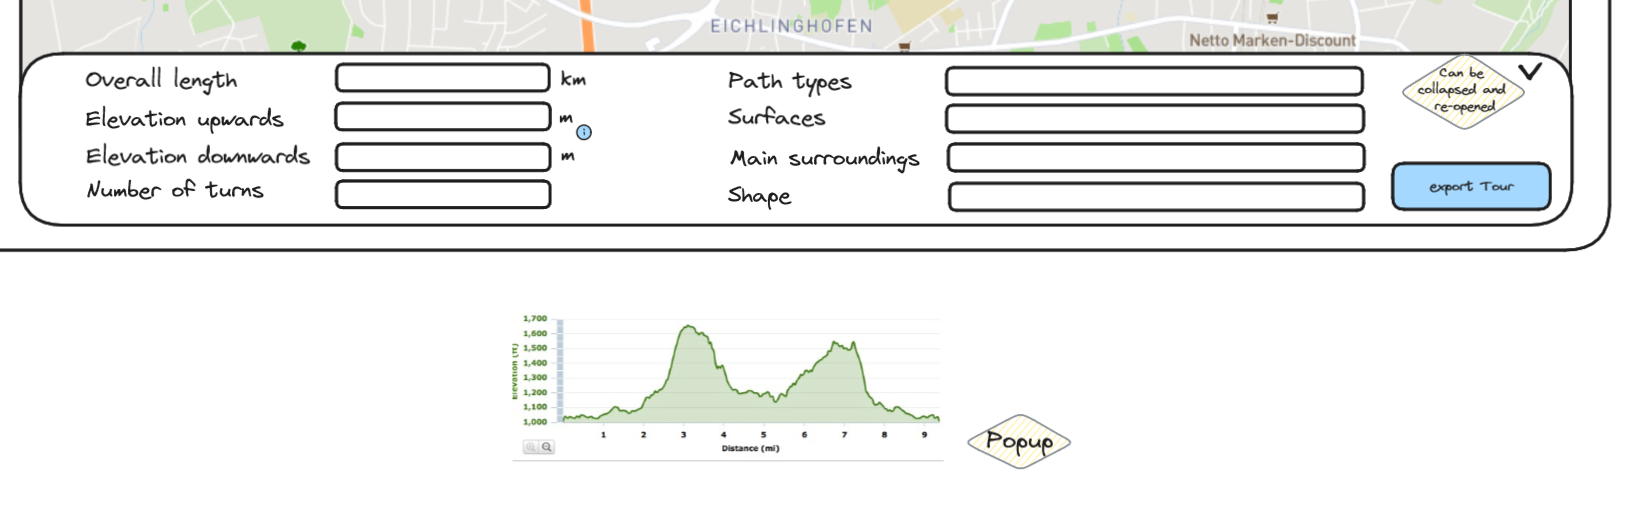
\includegraphics[width=0.9\linewidth]{bilder/Concept closeup tour stats, elevation profile.png}
	\caption{Design concept for the front end view, closeup of the results view}
	\label{fig:frontendConceptResultsCloseup}
\end{figure}



\section{Algorithmic changes}
\label{sec:algorithmicChanges}

\subsection{Ant Colony}
\label{subsec:antColonyImplementation}

\subsection{Genetic Algorithms}
\label{subsec:geneticAlgorithmsImplementation}

\subsection{Simulated Annealing}
\label{subsec:simulatedAnnealingImplementation}

\section{Parameter changes}
\label{sec:parameterChanges}


% kapitel2.tex
\chapter{Evaluation}
\label{chapter:evaluation}

This chapter presents a comprehensive analysis of the overall performance of Ant Colony, SA, and their implemented combinations.
In this analysis, several different parameter combinations are tested to achieve results of high quality.
The performance of Ant Colony is influenced by various parameters that could be changed and tested. 
However, analyzing all possible options would exceed the scope of this thesis.
Thus, the most important parameters with the highest impact on the results have been chosen.
For SA, most variables could be tested in different combinations, however, the way a neighborhood was constructed has not been varied at all, since only two different options have been implemented (using a probability distribution or picking Waypoints randomly).
Furthermore, the implemented combinations of Ant Colony with Greedy and MinCost, as well as the combinations of SA with Greedy, MinCost, and Ant Colony have been analyzed in comparison to each other. 


For both Ant Colony and SA, determining the number of outer loops as well as the number of ants per outer run for Ant Colony and the number of repetitions per outer run for SA are crucial parameters.
Furthermore, using the variables that can be changed by the user (importances of covered area, elevation, and edge profit) and analyzing their impact on the respective value as well as the overall quality are interesting factors to examine.
Thus, these test cases are performed for both algorithms.

First, the number of outer runs that are needed to achieve relatively good results for both algorithms (see pseudocode \ref{alg:AntColonyImplementation} and \ref{alg:SAImplementation} respectively) is determined.
Next, the inner loops and how the number of ants or the number of inner repetitions affects the quality are analyzed.
Additionally, the impact of each quality feature (covered area, edge profit and elevation) depending on the respective importance is visualized.
Lastly, the influence of each of these features on the quality is analyzed as well.

To achieve the following graphs, 30 test runs were conducted per varied variable unless stated otherwise.
The number of test runs is relatively small since conducting more tests per value would have been too time consuming.
Due to this small number of trials, the median results are presented and described.
However, for most cases, the average results are additionally presented in the appendix.
For both algorithms, to determine the number of outer runs, 100 test cases were conducted, making the average results more reliable.
Thus for these two cases, the average graphs were plotted.

For every case, the used base parameters that have not been varied are described in the corresponding paragraphs.
Some parameters remained constant across all test runs, specifically:

\begin{itemize}
	\item The starting point in front of Otto-Hahn-Straße 14
	\item The tour length of 4000m
	\item The desired tags for path type, surface, and surroundings
	\begin{itemize}
		\item Path type: asphalt
		\item Surface: paved, cobblestone, gravel, unpaved, compacted, fine gravel, rock, and pebblestone
		\item Surroundings: forest: tree
	\end{itemize}
	\item A maximum elevation of 100m
	\item A maximum steepness of 100\% 
	\item For Ant Colony, additional parameters include:
	\begin{itemize}
		\item The evaporation rate of 0.4
		\item The scaling value for penalties, in case a penalty was needed (e.g. using an edge twice) of 100
		\item The initial trail intensity of 0.0001
		\item The pheromone amount every ant can place per edge of 10
	\end{itemize}
	\item For SA, additional parameters include: 
	\begin{itemize}
		\item The initial temperature value of 0.9
		\item The number of Waypoints used to split up initial solutions of 10
	\end{itemize}
\end{itemize}

The choice for the steepness was made due to the coarse grained elevation values.
The inaccuracy of this data resulted in many parts with a calculated steepness exceeding 100\% which did not represent the reality.
Therefore, a high percentage was chosen to minimize the influence of the inaccurate data.

In all graphs, the x-axis represents the varied parameter and the y-axis shows the resulting values that will be analyzed.
Only for Ant Colony, test runs with two varied parameters (namely $\alpha$ and $\beta$) were conducted.
In these cases, the x- and y-axes show the varied parameters and the z-axis shows the resulting values that will be analyzed.
To provide a clearer overview of the results, several different views for these cases have been created.


\section{Ant Colony}
%
%To calculate a solution with Ant Colony, several variables have to be selected for the various calculations (see sections \ref{subsec:antColonyBackground} and \ref{subsec:antColonyImplementation}). 
%The relevant equations are listed below.
%All parameters that had to be set to a fitting value are highlighted in bold:
%
%\begin{align}
%		\Delta\tau_{ij}^k &= l(i,j) \cdot p(i,j) \cdot\textbf{ Q }\text{ if (i,j)} \in \text{tour collected by the ant}\\
%		\begin{split}
%			\nu_{ij}^k &= \boldsymbol{i_A} \cdot 100 \cdot \frac{\sqrt{|A|\cdot \pi} \cdot 2 }{L} 
%			+  \boldsymbol{i_p} \cdot 100 \cdot p
%			+ \boldsymbol{i_e} \cdot \left(\frac{e_{max} - e}{e_{max}} + \frac{s_{max} - s}{s_{max}}\right)
%		\end{split}\\
%			p_{ij}^k &= \begin{cases}
%			\frac{[\tau'_{ij}(t)]^{\boldsymbol{\alpha}} \cdot [\nu_{ij}]^{\boldsymbol{\beta}}}{\sum_{k \in allowed_k} [\tau'_{ij}(t)]^{\boldsymbol{\alpha}} \cdot [\nu_{ij}]^{\boldsymbol{\beta}}} &\text{if $j \in allowed_k$ }\\
%			0 &\text{otherwise}
%		\end{cases}
%\end{align}
%	
%The pheromone amount to be placed ($\Delta\tau_{ij}^k$) is based on the edgeProfit $p(i,j)$ (see Equation \ref{eq:newProfitCalc}) the edge with the length $l(i,j)$ will grant the tour
%The length $l(i,j)$ of the edge from node \textit{i} to node \textit{j} is multiplied by the profits $p(i,j)$ the same edge can collect based on the assigned tags, which is multiplied with the pheromone amount $Q = 10$, a single ant can place on the trail.


For Ant Colony, the initial test cases focused on finding good values for $\alpha$ and $\beta$, as these two parameters significantly influenced all following results.
After determining suitable values for $\alpha$ and $\beta$, the test cases outlined in the introduction, i.e. the number of outer runs, ants per run, and impact of the importances on the respective value and the overall quality, were performed.

The visibility for Ant Colony is calculated based on the respective importances for covered area ($i_A$), edge profit ($i_p$), and elevation and steepness ($i_e$).
These parameters are varied in increments of 0.1 for one optimization option in all cases where the importance is plotted.
When plotting the covered area importance, the importances of the edge profit and elevation are set to half of the remaining importance.
For example, if covered area importance of 0.2 is selected, the remaining importance is 0.8 and thus, the importance for edge profit and elevation are each set to 0.4.



\paragraph{\boldmath${\alpha}$ and \boldmath${\beta}$}

Before running any test cases on user-defined parameters, fitting values for $\alpha$ and $\beta$ need to be determined.
These parameters influence the probability of choosing an edge and impact the entire algorithm.
All test cases were performed with 100 ants per run and 25 outer iterations, with the importances set to 0.33 each. 
According to Dorigo et al. \cite{dorigo_ant_1996}, the values of $\alpha$ and $\beta$ should be in the range of $[0.5,5]$.
To identify good values, five scenarios were created:
\begin{itemize}
	\item $\beta$ set to 1 and $\alpha$ varying in $[0.5, 5]$
	\item $\alpha$ set to 1 and $\beta$ varying in $[0.5, 5]$
	\item Both $\alpha$ and $\beta$ varying in $[0.5, 5]$
	\item $\beta$ set to 1.5 and $\alpha$ varying in $[0.5, 5]$
	\item $\alpha$ set to 0.8 and $\beta$ varying in $[0.5, 5]$
\end{itemize}


For the five listed cases, the corresponding graphs are visualized in Figures \ref{fig:antColonyCasesAlphaVariedMed} to \ref{fig:antColonyCasesBetaVariedAlpha08} and additional visualizations can be found in the appendix (Figures \ref{fig:antColonyCasesAlphaVariedAvg} to \ref{fig:antColonyCasesAlphaAndBetaVariedAvgAll}).
The first Figure (\ref{fig:antColonyCasesAlphaVariedMed}) shows the median quality results of 30 test runs for $\beta = 1$ per $\alpha$, where the steps started in 0.1 increments between 0.5 and 1.0 and then continued in 0.5 increments from 1.0 to 5.0.


\begin{figure}
	\centering
	\includesvg[width=0.9\textwidth]{bilder/plots/AntFinal/antColonyCasesAlphaVariedMed.svg}
	\caption{Ant colony median quality values over varied $\alpha$, $\beta = 1$}
	\label{fig:antColonyCasesAlphaVariedMed}
\end{figure}


The results as shown in Graph \ref{fig:antColonyCasesAlphaVariedMed} indicate that for a constant $\beta = 1$, the best outcomes can be achieved with a low $\alpha$ between 0.5 and 2.0, and with $\alpha = 3.5$.

Similarly, the second figure displays results for $\alpha = 1$ and a varying $\beta$.
Again, between 0.5 and 1.0, the steps on the x-axis increased by 0.1, and by 0.5 from 1.0 to 5.0.


\begin{figure}
	\centering
	\includesvg[width=0.9\textwidth]{bilder/plots/AntFinal/antColonyCasesBetaVariedMed.svg}
	\caption{Ant colony median quality values over varied $\beta$, $\alpha = 1$}
	\label{fig:antColonyCasesBetaVariedMed}
\end{figure}

Graph \ref{fig:antColonyCasesBetaVariedMed} indicates that a low $\beta$ of  $0.5, 1.5$, or $\beta = 3.5$ could yield good results.
However, since both graphs have a constant second variable, the results could be dependent on the respective value.
To get a better overview over the effects of both $\alpha$ and $\beta$, additional test cases were run where both variables varied in the interval $[0.5, 5]$.
Again, the step size between 0.5 and 1.0 was 0.1 and the step size between 1.0 and 5.0 was 0.5.

The applied color map highlights low values in blue and purple, middling values in magenta and pink, and high values in orange and yellow.
%Blue being the lowest and yellow the highest values.
In the top subfigure, the different points of the median of all test cases can be seen.
The two figures below show a surface plot of the same test case, Subfigure \ref{fig:antColonyCasesAlphaAndBetaVariedMedSurface} in a side view, and Subfigure \ref{fig:antColonyCasesAlphaAndBetaVariedMedTopDown} in a top-down view. 
All three figures show yellow points for a combination of very low $\alpha$ and low $\beta$ values with $\alpha < 1.0$ and $\beta \leq 3.0$, for very high values of $\beta$ ($\beta \geq 4.0$) and $\alpha$ values in a range of $2 \leq \alpha \leq 4.5$, and one high value for $\alpha = 5$ and $\beta = 2.5$.

\begin{figure}
	\begin{subfigure}{0.48\textwidth}
		\includesvg[width=\textwidth]{bilder/plots/AntFinal/antColonyCasesAlphaAndBetaVariedSurfaceMed.svg}
		\caption{Ant colony median quality values over varied $\alpha$ and $\beta$ surface plot}
		\label{fig:antColonyCasesAlphaAndBetaVariedMedSurface}
	\end{subfigure}
	\hfill
	\begin{subfigure}{0.48\textwidth}
		\includesvg[width=\textwidth]{bilder/plots/AntFinal/antColonyCasesAlphaAndBetaVariedSurfaceMedTopDown.svg}
		\caption{Ant colony median quality values over varied $\alpha$ and $\beta$ surface plot top-down view}
		\label{fig:antColonyCasesAlphaAndBetaVariedMedTopDown}
	\end{subfigure}
	\caption{Plot of varied $\alpha$ and $\beta$ in different views}
	\label{fig:antColonyCasesAlphaAndBetaVariedMedAll}
\end{figure}



The median quality plots in Graph \ref{fig:antColonyCasesAlphaAndBetaVariedMedAll} provide several potential options for $\alpha$ and $\beta$. 
However, the plots of the average qualities (see Figure \ref{fig:antColonyCasesAlphaAndBetaVariedAvgAll}) show a peak at $\alpha = 0.8$ and $\beta = 1.5$, aligning with one of the options shown in the median quality plots in Figure \ref{fig:antColonyCasesAlphaAndBetaVariedMedAll}.

Furthermore, tests with $\alpha$ set to 0.8 and a varying $\beta$ as well as with $\beta$ set to 1.5 and a varying $\alpha$ have been conducted.
The results are shown in Figures \ref{fig:antColonyCasesAlphaVariedBeta15} and \ref{fig:antColonyCasesBetaVariedAlpha08}.


\begin{figure}
	\centering
	\includesvg[width=0.9\textwidth]{bilder/plots/AntFinal/antColonyCasesAlphaVariedBeta15Med.svg}
	\caption{Ant colony median quality values over varied $\alpha$, $\beta = 1.5$}
	\label{fig:antColonyCasesAlphaVariedBeta15}
\end{figure}

\begin{figure}
	\centering
	\includesvg[width=0.9\textwidth]{bilder/plots/AntFinal/antColonyCasesBetaVariedAlpha08Med.svg}
	\caption{Ant colony median quality values over varied $\beta$, $\alpha = 0.8$}
	\label{fig:antColonyCasesBetaVariedAlpha08}
\end{figure}


The plots in Graphs \ref{fig:antColonyCasesAlphaVariedBeta15} and \ref{fig:antColonyCasesBetaVariedAlpha08} show that for a constant $\beta$ of 1.5, higher quality values can be found for $ 0.6 \leq \alpha \leq 0.8$ and $\alpha = 4$.
Of these possible options, the peak for $\alpha = 0.8$ matches the results of Figures \ref{fig:antColonyCasesAlphaAndBetaVariedMedAll}.
More high values present in the second plot (see Figure \ref{fig:antColonyCasesBetaVariedAlpha08}) where $\alpha$ was set to 0.8:
For $\beta = 0.6$ , $0.9 \leq \beta \leq 1.5$ and $3.5 \leq \beta \leq 4$, high quality values are returned.
Of these possible options, the peak for $\beta = 1.5$ matches the results of Figure \ref{fig:antColonyCasesAlphaAndBetaVariedMedAll}, highlighting that these choices result in a higher quality of the returned tour.
Based on these results, $\alpha$ and $\beta$ were chosen to be set to $\alpha = 0.8$ and $\beta = 1.5$ for the following test cases.


\paragraph{Quality Over Runs}

The next conducted test (see Figure \ref{fig:AntColonyQualityRuns}) visualizes how many runs of the outer loop of Ant Colony are needed before the quality increase slows to a plateau. 
The respective figure shows the results of the average quality values from 100 tests per outer loop run, each executed with 100 ants. 
The \enquote{Run}-axis displays the number of runs in the outer loop, while the \enquote{Quality}-axis indicates the resulting quality value.


\begin{figure}
	\centering
	\includesvg[width=0.9\textwidth]{bilder/plots/AntFinal/antColonyCasesNumberRunsQualityAvgWithoutFittedLine.svg}
	\caption{Ant colony average quality values over runs}
	\label{fig:AntColonyQualityRuns}
\end{figure}

%\begin{figure}[H]
%	\includesvg[width=0.9\textwidth]{bilder/plots/antColonyCasesNumberRunsQualityAvg.svg}
%	\caption{Ant colony quality over runs (average)}
%	\label{fig:AntColonyQualityRunsLogFunc}
%\end{figure}

Figure \ref{fig:AntColonyQualityRuns} shows a steep increase in quality for 1 to 5 runs.
After this initial phase, the increase slows to a near plateau and remains relatively even for the subsequent runs. 
The graph indicates that after 10-15 runs, no significant increase in quality is achieved, even with a larger number of runs. 
Thus, 20 iterations were deemed to be sufficient for generating good results in the following test cases.


Next, the number of ants and how they impact the quality of a given solution was examined. 
Graph \ref{fig:AntColonyQualityAnts} displays the median quality values of the results of 30 test runs per selected number of ants.
Notably, some outliers of exceptionally high qualities are evident with fewer ants. 
These outliers are more apparent in the plot that shows all runs (see Figure \ref{fig:AntColonyQualityAntsAll} in the appendix).
However, the increase in median quality values from 100 to 500 ants demonstrates that, overall, more ants result in better outcomes.

For the following use cases, 100 ants were selected, since the case with 100 ants was the first that did not show a single outlier, but several higher quality values and a relatively high median value. 
Although using more ants improves the results, the run time, which is already relatively long for just 100 ants and the selected 20 iterations, also increases. 

%(see Figure \ref{fig:}) \#TODO add time plot!!!


\begin{figure}
	\centering
	\includesvg[width=0.9\textwidth]{bilder/plots/AntFinal/antColonyCasesNumAntsMed.svg}
	\caption{Ant colony median quality values over number ants}
	\label{fig:AntColonyQualityAnts}
\end{figure}




\paragraph{Covered Area}

To analyze the impact of the covered area importance on both the resulting covered area and general quality, several tests were conducted.
The first Figure (\ref{fig:AntColonyAreaMed}) shows the median covered area results for 30 test runs per importance value and the respective lines of best fit for the covered area importance values.
The second Figure (\ref{fig:AntColonyAreaQualityMed}) shows the results of the median quality values with the same configuration.
Graphs displaying the respective average values can be found in the appendix (see \ref{fig:AntColonyAreaAvg} and \ref{fig:AntColonyAreaQualityAvg}).

\begin{figure}
	\centering
	\includesvg[width=0.9\textwidth]{bilder/plots/AntFinal/antColonyCasesCoveredAreaMed.svg}
	\caption{Ant colony median covered area values over covered area importance}
	\label{fig:AntColonyAreaMed}
\end{figure}

\begin{figure}
	\centering
	\includesvg[width=0.9\textwidth]{bilder/plots/AntFinal/antColonyCasesCoveredAreaQualityMed.svg}
	\caption{Ant colony median quality values over covered area importance}
	\label{fig:AntColonyAreaQualityMed}
\end{figure}

Graph \ref{fig:AntColonyAreaMed} highlights that increasing the importance of the covered area, correlates with higher returned area values.
Only in the case of a single ant does the graph show a decrease, indicating that with one ant, the randomness is too great to achieve the expected results.
This observation is underscored by the plotted points (blue), which oscillate significantly between high and low values.
For all other cases (10, 50, and 100 ants), an increase in covered area is observed.
With the steepest increase for 100 ants, resulting in the highest returned area values for an importance of $\geq 0.4$.


Graph \ref{fig:AntColonyAreaQualityMed} illustrates how the quality changes with varying importance for the covered area.
In this visualization, a substantial increase in quality can be observed for 1 and 10 ants, a slight increase for 50 ants, and a decrease for 100 ants.
This development suggests that the covered area is not the most impactful value in determining the quality.
Since overall quality is used to calculate the probability of choosing the next point during tour creation, this development indicates, that Ant Colony is negatively affected by a high importance of the covered area.


This result changes, when only the covered area is considered and both elevation importance and edge profit importance are set to 0 (see Figure \ref{fig:AntColonyAreaOnlyQualityMed}).
In the respective graph, with increasing covered area importance, the overall quality increases, indicating that neither the edge profit nor the elevation change impacts the quality, as was expected.


\begin{figure}
	\centering
	\includesvg[width=0.9\textwidth]{bilder/plots/AntFinal/antColonyCasesCoveredAreaOnlyQualityMed.svg}
	\caption{Ant colony median quality values over covered area importance, elevation importance and edge profit importance both set to 0}
	\label{fig:AntColonyAreaOnlyQualityMed}
\end{figure}

Overall, these results show that while the covered area does impact the quality, edge profit and elevation have a much more significant impact on the overall result.
This larger impact is expected, as ants typically choose the next edge with the highest probability.
The probability is calculated using covered area, elevation, and edge profit, but the current quality increase is valued higher than the overall quality increase.

All of the graphs show that quality values are lower when more ants are used.
However, the covered area is generally larger with more ants -- especially when considering extreme points.
The graph analyzing the influence of the number of ants on the quality (Figure \ref{fig:AntColonyQualityAnts}) shows, that there are many fluctuations with fewer ants.
Thus, although the quality seems mostly lower, using 100 ants yields more reliably good results.

\paragraph{Elevation}


To analyze the impact of the elevation importance on both the resulting elevation and on the general quality, several tests were conducted.
The first Figure (\ref{fig:AntColonyElevationMed}) shows the median elevation results for 30 test runs per importance value along with the respective lines of best fit for the elevation importance values.
The second figure (\ref{fig:AntColonyQualityElevationMed}) shows the results of the median general quality values with the same configuration.
Graphs displaying the respective average values can be found in the appendix (see figures \ref{fig:AntColonyElevationAvg} and \ref{fig:AntColonyQualityElevationAvg}).


\begin{figure}
	\centering
	\includesvg[width=0.9\textwidth]{bilder/plots/AntFinal/antColonyCasesElevationMed.svg}
	\caption{Ant colony median elevation values over elevation importance}
	\label{fig:AntColonyElevationMed}
\end{figure}



\begin{figure}
	\centering
	\includesvg[width=0.9\textwidth]{bilder/plots/AntFinal/antColonyCasesElevationQualityMed.svg}
	\caption{Ant colony median quality values over elevation importance}
	\label{fig:AntColonyQualityElevationMed}
\end{figure}


Graph \ref{fig:AntColonyElevationMed} highlights that as the importance of the elevation increases, the returned elevation value also rises. 
For this case, the returned values are not height meters but describe the elevation measure used in the quality calculation (see Equation \ref{eq:visibility}).
Similarly to the covered area, using fewer ants results in a slightly decreasing value when the importance is increased. 
This graph shows a downward slope for 1 and 10 ants and only a very slight increase for 50 ants.
The only case that shows a definitive increase with higher importance is the one where 100 ants are used.
Again, this behavior as well as the fact that the overall elevation measure is the lowest for the 100 ants can be explained by a less varying result which does not have as many outliers.


Graph \ref{fig:AntColonyQualityElevationMed} shows that for higher elevation importance the quality also increases.
In this visualization, all qualities increase with the importance.
Furthermore, the result for 100 ants has the second highest quality results.
With rising elevation importance values, the quality increases, indicating that elevation has a larger impact on the quality than the covered area when using the Ant Colony algorithm. 




\paragraph{Edge Profit}

To analyze the impact of the edge profit importance on both the resulting edge profit and on the general quality, several tests were conducted.
The first Figure (\ref{fig:AntColonyProfitMed}) shows the median edge profit results for 30 test runs per importance value, along with the respective lines of best fit for the edge profit importance values.
The second Figure (\ref{fig:AntColonyQualityProfitMed}) shows the results of the median quality values with the same configuration.
Graphs displaying the respective average values can be found in the appendix (see figures \ref{fig:AntColonyProfitAvg} and \ref{fig:AntColonyQualityProfitAvg}).


\begin{figure}
	\centering
	\includesvg[width=0.9\textwidth]{bilder/plots/AntFinal/antColonyCasesProfitMed.svg}
	\caption{Ant colony median edge profit values over edge profit importance}
	\label{fig:AntColonyProfitMed}
\end{figure}


\begin{figure}
	\centering
	\includesvg[width=0.9\textwidth]{bilder/plots/AntFinal/antColonyCasesProfitQualityMed.svg}
	\caption{Ant colony median quality values over edge profit importance}
	\label{fig:AntColonyQualityProfitMed}
\end{figure}


Graph \ref{fig:AntColonyProfitMed} highlights that higher importance of the edge profit, results in increased edge profit values. 
Again, this increase is only evident when 100 ants are used. 
With fewer ants, the importance decreases the resulting edge profit values.
These results, as well as the fact that the resulting profit is again lower than for fewer ants, are due to the higher variability when fewer ants are used.
For 100 ants, increasing the edge profit importance results in higher edge profits.


Graph \ref{fig:AntColonyQualityProfitMed} shows that for 100 ants, the quality increases significantly with the importance of the edge profit.
For fewer ants, the results are more mixed.
For 1 and 50 ants, a significant decrease can be seen.
For 10 ants, the quality increases slightly.
These results highlight how variable the returned quality is when only a few ants are used.
The result for the 100 ants fits into the results for the covered area, showing that the edge profit is more important for the resulting quality than the covered area. 
Both the elevation and the edge profit increase the quality when their importances are increased.
However, the edge profit graph shows that the overall quality is mostly lower when more ants are used.
This behavior is equivalent to the graph for elevation values.


Overall, all graphs show that all three user-defined values contributing to the quality rise with an increase in their respective importance.
The quality only decreases for high covered area importances.
The overall resulting tour does take the selected user preferences, which correspond to the importances into account.
All in all, the graphs show that with fewer ants, high variability can cause results that do not match expectations.
However, for the selected 100 ants, all cases display the expected behavior.
Furthermore, the test cases have shown that for Ant Colony to achieve good results, the covered area is less important than the elevation and edge profits.
This result can be attributed to the fact that for every single ant, the decision of which edge to choose is local.
Thus, both the elevation and the edge profit have a larger weight than the covered area, which is a more global variable.


\section{Simulated Annealing}

%To calculate a solution, several variables have to be selected for the various calculations (see sections \ref{subsec:simulatedAnnealingBackground} and \ref{subsec:simulatedAnnealingImplementation}). 
%First, a temperature function had to be determined.
%Then, like for the ant algorithm, the importances will be tested and the results displayed.
%Furthermore, the number of inner runs has to be set.
%For these cases, 10 inner runs have been performed.

For SA, the initial test cases focused on determining a good temperature function. 
The rate at which the temperature decreases is crucial as this development significantly influences the probability of accepting a worse solution, making this parameter the most vital variable to configure.
Four different functions were selected based on the options presented in Section \ref{subsec:simulatedAnnealingBackground}:

\begin{itemize}
	\item $	T_{i+1} = \frac{- |f(j)-f(i)|}{ln(r_i)}	$
	\item $T_{i+1} = 0.5 \cdot T_i$
	\item $T_{i+1} = e^{-2} \cdot T_i$
	\item $T_{i+1} = \frac{T_i}{1 + T_i}$
\end{itemize}

The test cases were executed according to the parameters outlined in this chapter's introduction, including the number of outer iterations, inner repetitions, and the influence of the importances on the respective variables and the overall quality.
For SA, the user-defined importances are incorporated into the quality calculation and consistently impact the returned results.


The tests for the needed number of runs and the determination of a suitable temperature function have been executed in the same test case.
For the importances, three cases have been constructed and executed, the same way the tests have been done for Ant Colony.
The evaluation for the necessary number of runs and the suitable temperature function as well as for the importances were concluded and tested following the same methodology used for Ant Colony tests.


\paragraph{Quality Over Runs and Repetitions}

To determine a good number of runs and a fitting temperature function for achieving relatively good results, the median quality over number of runs performed has been plotted for the four different temperature functions in Figure \ref{fig:SAQualityRuns}.
The respective figure presents the average quality values from 100 test runs per outer loop run, each using 10 inner repetitions with importances of 0.33 each.
The \enquote{Run}-axis displays the number of runs in the outer loop, while the \enquote{Quality}-axis shows the resulting quality value.

\begin{figure}
	\makebox[\textwidth][c]{
	\includesvg[width=1.2\textwidth]{bilder/plots/SAFinal/SACasesTempFctionAvg.svg}}
	\centering
	\caption{SA average quality values over runs}
	\label{fig:SAQualityRuns}
\end{figure}

Figure \ref{fig:SAQualityRuns} presents several important findings:
First, calculating the temperature using a multiplying factor -- in this case $e^{-2}$ -- yields the best resulting quality.
Furthermore, for most functions, a plateau is reached after 200 runs, except for the function denoted as $ T_{i+1} = \frac{- |f(j)-f(i)|}{ln(r_i)} $ (green).
This function does not improve the quality at all, but rather remains relatively stable with some outliers where the quality increases temporarily.
In all other cases, where quality improvements occur, there are noticeable \enquote{steps} where the quality remains consistent for a few runs before increasing again.
These steps are most noticeable in the yellow curve but are also evident in the blue and red graphs.
This stepping behavior arises because the SA tends to find local optima.
The algorithm can eventually escape these local optima with more runs.
The obvious steps indicate where these local optima occur.
Furthermore, these steps often overlap across the different temperature functions.



Using more internal repetitions increases the quality (see Figure \ref{fig:SAQualityRepititions}), but also inevitably significantly increases the run time.
Given that the first figure shows a plateau at 250 runs and using 10 repetitions already yielded a median runtime of 22 seconds (see Figure \ref{fig:SATimeOverRuns}), using more internal repetitions would have increased the runtime excessively.
Based on these results, the following tests have been performed with the temperature function that yielded the best results ($T_{i+1} = e^{-2} \cdot T_i$), 10 internal repetitions, and 250 runs.


\paragraph{Covered Area}

To analyze the impact of the covered area importance on both the resulting covered area and on the general quality, several tests were conducted.
The first Figure (\ref{fig:SAAreaMed}) shows the median covered area results for 30 test runs per importance value, along with the respective lines of best fit for the covered area importance values.
The second Figure \ref{fig:SAAreaQualityMed} presents the median results for overall quality with the same configuration.
Graphs displaying the respective average values can be found in the appendix (see \ref{fig:SAAreaAvg} and \ref{fig:SAAreaQualityAvg}).



\begin{figure}
	\centering
	\includesvg[width=0.9\textwidth]{bilder/plots/SAFinal/SACasesNumberRunsCoveredAreaMed.svg}
	\caption{Simulated Annealing median covered area values over covered area importance}
	\label{fig:SAAreaMed}
\end{figure}

\begin{figure}
	\centering
	\includesvg[width=0.9\textwidth]{bilder/plots/SAFinal/SACasesNumberRunsCoveredAreaQualityMed.svg}
	\caption{Simulated Annealing median quality values over covered area importance}
	\label{fig:SAAreaQualityMed}
\end{figure}


Graph \ref{fig:SAAreaMed} highlights that the higher the importance of the covered area, the higher the returned area values.
For 1, 5, and 10 runs, the covered area is significantly lower than for 50, 100, and 250 runs causing the three resulting lines of best fit for fewer runs to overlap.
In the three cases with larger resulting covered area values, an increase can be seen as the importance value rises.
Most importantly, for SA, the more runs that are performed, the higher the returned area values generally are.


Graph \ref{fig:SAAreaQualityMed} shows how the quality changes with a varying importance for the covered area.
Here, the results for 1, 5, and 10 runs all overlap because the quality values are too low to be distinctly visible, similarly to the figure displaying the results for covered area.
For 250 runs, a slight increase in the resulting quality can be seen, however, with fewer runs, the quality mostly decreases as the importance of the covered area nears 100\%.
This behavior indicates that with fewer runs, the area can negatively impact the resulting quality.
However, for 250 runs, the impact is distinctly positive, showing that the covered area is relatively important for the quality of SA.


\paragraph{Elevation}

To analyze the impact of the elevation importance on both the resulting elevation and on the general quality, several tests were conducted.
The first Figure \ref{fig:SAElevationMed} shows the median elevation results for 30 test runs per importance value, along with the respective lines of best fit for the elevation importance values.
The second Figure \ref{fig:SAQualityElevationMed} presents the results of the median general quality values with the same configuration.
Graphs displaying the respective average values can be found in the appendix (see figures \ref{fig:SAElevationAvg} and \ref{fig:SAQualityElevationAvg}).



\begin{figure}
	\centering
	\includesvg[width=0.9\textwidth]{bilder/plots/SAFinal/SACasesNumberRunsElevationMed.svg}
	\caption{Simulated Annealing median elevation values over elevation importance}
	\label{fig:SAElevationMed}
\end{figure}



\begin{figure}
	\centering
	\includesvg[width=0.9\textwidth]{bilder/plots/SAFinal/SACasesNumberRunsElevationQualityMed.svg}
	\caption{Simulated Annealing median quality values over elevation importance}
	\label{fig:SAQualityElevationMed}
\end{figure}

Graph \ref{fig:SAElevationMed} shows that the elevation importance does not change the elevation resulting values at all.
Instead, all results converge to the same value when considering the median. 
In the average graph, this development does look slightly different, however, this result shows, that the elevation does not have a significant impact.
This smaller impact could be due to the selected starting point.
Given that the SA with an empty starting solution and a probability function was used for all test runs, the possibility arises, that the probability functions did not offer many different options within the selected area, resulting in most returned paths having the same elevation values regardless of the number of runs or of the importance level chosen.
In the average graph (see Figure \ref{fig:SAElevationAvg}), there is a slight increase in the elevation value for most runs.
The results for 10 and 50 runs are slightly decreasing, which could be due to not performing enough runs to reach a solution that better fits the chosen importances.
However, the overall area where the tests were performed limits the available options, leading to minimal variability in the elevation values.
All results are between 0.43 and 0.49, indicating very similar elevation values overall.


Graph \ref{fig:SAQualityElevationMed} shows that for the elevation importance, the quality distinctly increases, especially for 100 and 250 runs. 
The results for 1, 10, and 50 runs overlap for this case as well.
The increase in quality can be attributed to the lower importance of the edge profits and covered area, which increase the influence of the elevation result, indicating that the returned elevation result has already been very good.



\paragraph{Edge Profit}


To analyze the impact of the edge profit importance on both the resulting edge profit as well as on the general quality, several tests were conducted.
The first Figure (\ref{fig:SAProfitMed}) shows the median edge profit results for 30 test runs per importance value and the respective lines of best fit for the edge profit importance values.
The second Figure (\ref{fig:SAQualityProfitMed}) shows the results of the general quality values with the same configuration.
Graphs displaying the respective average values can be found in the appendix (see figures \ref{fig:SAProfitAvg} and \ref{fig:SAQualityProfitAvg}).


\begin{figure}
	\centering
	\includesvg[width=0.9\textwidth]{bilder/plots/SAFinal/SACasesNumberRunsProfitMed.svg}
	\caption{Simulated Annealing median edge profit values over edge profit importance}
	\label{fig:SAProfitMed}
\end{figure}


\begin{figure}
	\centering
	\includesvg[width=0.9\textwidth]{bilder/plots/SAFinal/SACasesNumberRunsProfitQualityMed.svg}
	\caption{Simulated Annealing median quality values over edge profit importance}
	\label{fig:SAQualityProfitMed}
\end{figure}




Graph \ref{fig:SAProfitMed} highlights that increasing the importance of the edge profit rises the returned edge profit values by a tiny amount. 
This increase is only prevalent for 250 runs, while for fewer runs, a slight, and for 50 runs even a steep decrease can be observed. 
As with the covered area, this development is most likely because not enough runs could be executed to reach a solution that results in an increase in the edge profits and the quality.
Overall, the changes are within a very small spectrum of possible results, with most graphs varying by less than 0.0001 and only the graph for 50 runs varying by 0.0003.
This highlights the results of the elevation graphs, that not much variability was possible for the specific configuration used for testing.


Graph \ref{fig:SAQualityProfitMed} shows that for 250 repetitions, the quality decreases with the importance of the edge profit.
For fewer repetitions, the resulting qualities stay on a relatively even level.
In the respective average plot (see Figure \ref{fig:SAQualityProfitAvg}), this decrease and the difference in total value between the quality result for an edge profit importance of 0.1 and an edge profit importance of 1.0 is not as large as in the median plot.
The overall quality is, however, still decreasing.
This result highlights that for Simulated Annealing, optimizing for the edge profit negatively impacts the overall quality. 
Especially when viewed in combination with the results for the covered area, this finding indicates that the edge profits are less relevant for achieving high quality outcomes using SA.



Overall, all graphs demonstrate that the three user defined importances contribute to a respective rise of the returned value in the resulting tour.
The covered area increases the quality slightly, while the edge profits cause a slight decrease.
This behavior implies that the more global variable covered area is more important for the quality of Simulated Annealing, which overall focuses on optimizing a global result.
The elevation had a significant impact for the given test case, likely because the elevation result was generally very good for all calculated solutions, thus having a more positive impact as the elevation importance was valued higher.





\section{All Algorithms}

Lastly, all implemented algorithms, including the combinations, were evaluated across varying maximum run times. 
Each algorithm was configured as previously specified: 
For Ant Colony and the respective combinations, 100 ants were used, for SA and all respective combinations, 10 inner repetitions were selected.
All test cases were executed with equal importances of 0.33 for all the quality values.
The maximum run times tested were 1, 2, 5, 10, 15, 20, and 30 seconds, with each maximum time being tested over 30 test runs.

\begin{figure}
	\centering
	\includesvg[width=0.9\textwidth]{bilder/plots/All/AllCasesTimeQualityMed.svg}
	\caption{All implemented algorithms' median quality values over time}
	\label{fig:AllOverTime}
\end{figure}


Figure \ref{fig:AllOverTime} shows the median quality values of the 30 test runs for all algorithms per allowed maximum run time.
The ant algorithms, including both of their combinations did all produce low quality results compared to the Simulated Annealing ones and did not show a significant increase in quality. 
To better illustrate these changes, two separate graphs were plotted. 


\begin{figure}
	\centering
	\includesvg[width=0.9\textwidth]{bilder/plots/All/AllCasesAntTimeQualityMed.svg}
	\caption{All ant variants' median quality values over time}
	\label{fig:AllOverTimeAnt}
\end{figure}


Figure \ref{fig:AllOverTimeAnt} displays the performance of the three Ant Colony versions, using only Ant Colony or a combination with either the Greedy or the MinCost tour as a base.
Both combinations show a large improvement in quality over time, indicating that the base tours are optimized considerably by the ants.
However, the basic Ant Colony algorithm, only shows a slight quality increase.
Overall, all quality values are much lower than the SA results, even though an increase can be seen for all cases.

The results indicate that Ant Colony is not the most suited for finding a good tour.
Even though the algorithm does take all user configurations into account, the local decisions every ant made, result in a relatively low overall quality.



\begin{figure}
	\centering
	\includesvg[width=0.9\textwidth]{bilder/plots/All/AllCasesSATimeQualityMed.svg}
	\caption{All SA variants' median quality values over time}
	\label{fig:AllOverTimeSA}
\end{figure}


The final plot (Figure \ref{fig:AllOverTimeSA}) provides a more detailed comparison of the various SA implementations. 
In this graph, the \texttt{SimulatedAnnealingEmpty} is the standard SA algorithm used in all previous test cases.
This implementation started with an empty base tour and a probability configuration.
The fully random version also started with an empty tour but lacks a probability distribution for node selection.
The other three combinations used their respective referenced algorithm as base tours to optimize.

This graph indicates that the combination of MinCost and the SA algorithm did not significantly improve. 
However, using the shortest allowed run times, the result is still of much higher quality than the Ant Colony optimized one.
Furthermore, the empty solution with a probability distribution had the lowest overall quality, with only minor improvements over time.
The fully random version showed a slightly steeper increase but both algorithms that start with an empty configuration remained at the lowest quality level.
However, the combination with the Greedy base tour as well as with the Ant Colony have a very steep increase. 

Overall, the graphs show, that the combination of MinCost and Simulated Annealing results in a very good solution even for short run times.
The pink line that displays the results of this combination is the same as the results for MinCost alone (see Figure \ref{fig:AllGreedyMinCost}), indicating, that for the median of all results, no improvement could be made on the MinCost result.
However, the average graphs show a different behavior (see Figures \ref{fig:AllAverage} and \ref{fig:AllSAAverage}).
In these graphs, all SA variants exceed the quality of the MinCost result after a runtime of at most 12 seconds.
This different behavior for the averages indicates that there are some tours that can significantly improve the quality of MinCost, but not enough higher quality tours were calculated to achieve the same results in the median.
The varying results could be due to the starting point or other starting conditions such as the selected maximum elevation or the selected desirable tags.

 
While all other algorithms show some quality improvements over time, only the combination of Ant Colony and Simulated Annealing improves enough to exceed the quality of the MinCost-Simulated Annealing combination.
However, the results could look very differently for other importance combinations.
The MinCost algorithm starts with a tour that has a very high covered area value, greatly impacting the initial quality, which is then further enhanced by using Simulated Annealing.
When the covered area importance is set very low, using this combination can quickly result in a less optimal tour.


The conducted test cases do not cover all possible parameters, configurations and are far from covering all combinations.
For all algorithms, especially the combinations of Ant Colony and Simulated Annealing with other algorithms, several additional test cases are possible.
However, conducting more than the presented cases significantly exceeds the time frame of this thesis and thus has to be part of possible future work (see Section \ref{sec:futureWork}).















% kapitel2.tex
\chapter{Conclusion}
\label{chapter:conclusion}

In conclusion, the implementations of this thesis have achieved the goals set in the introduction (\ref{sec:goal}):
The previous version of Tour4Me was extended by both parameter options as well as two meta-heuristic approaches. 
Additionally, combinations of the two new meta-heuristics and the existing algorithms were implemented.
The front end was changed and matched to the added customization options, creating a better overview and improving the overall layout.
For most data-points and tour lengths, roundtrips can be created using at least one of the available algorithms. 
The only points that are no valid starting points are those outside the valid graph or without any connections to valid edges.

\section{Results}
\label{sec:results}




\section{Future Work}
\label{sec:futureWork}

For this thesis, several changes have been implemented to create an app that offers many customization options and also utilizes different algorithms to find roundtrips that are suited to the user preferences.
However, there are still many open ends to optimize and enhance the current solution.

First, there are not too many surrounding information available in the OSM data, despite the fact that the map visualization does have areas colored based on their surroundings.
Thus, the information are saved at some point and a means to extract them should exist.
Using the visualization or the data used to find the correct colors could enable a much wider coverage of points with respective surrounding information. 
Adding these tags will result in many more edges that can be labeled according to the kind of area they are placed in and thus result in a much better portray and filtering of the actual nodes.
Currently, the limited surrounding information make the chance of these data to impact a tour very slim.
Only about 8\% of the nodes in Germany can be matched to surrounding information\footnote{\url{https://dashboard.ohsome.org/}, last accessed: 03.06.2024}.

Additionally, the used elevation information could be upgraded to use a more fine grained database, resulting in more precise values. 
Currently, it is possible to end up with a steepness of over 100\% because of the inaccurate elevation information.
Better versions could be available from the NASA, however downloading and using them was a lot more complicated than the docker setup from open elevation.
A more detailed research for better data -- that also can be easily used and queried -- has to be done to determine a good solution for this problem.

Aside from fixing current data issues, several other enhancements and extensions are possible.
The number of parameters to change the user preferences can be increased. 
Especially for elevation information, several additional constraints could be used:
\begin{itemize}
	\item steepness split into ascending and descending values: This addition is very interesting for people with knee problems. Oftentimes steep ascensions are not a problem, but steep descends put too much strain on their knees. Thus, directed tours that can be bound for both steepness values separately can be extremely useful.
	\item adding more detailed options: currently, the overall elevation difference in the tour is calculated. However, many other information could be interesting:
	 A bound on how long any part of the tour is allowed to constantly ascend or descend. This could again be split into two variables.
	Additionally, the maximum ascend per 50, 100 or 1000 m could be more interesting than a maximum steepness of any small part.
	\item a visualization of the height profile of the tour: this is mainly a front end extension, but depending on the needed data, the way paths are saved might need to be changed to allow for saving and returning elevation information of the tour for this visualization
\end{itemize}

Furthermore, many other algorithms -- especially different meta-heuristics -- could be implemented. 
One particularly interesting approach could be using a genetic algorithm.
For this, only the genetic algorithm itself as well as several combinations could be interesting. 
These combinations would demand much more changing than the current combinations, since generations of the algorithms have to be created, mutated and thus optimized. 
To realize genetic changes, several possible approaches can be thought of. 
For a combination with the ant algorithm, changing the ant parameters and having the ants with the best results survive and create offspring could greatly increase the quality of the ant solutions.
Combining with SA to try out different temperatures and cooling schedules, different methods of creating neighboring solutions, or many other base operations could be interesting.
Again, this combination could yield very different and possibly much better resulting tours.

Aside from these extensions, the runtime is a main part of the implementation that could be enhanced by a lot. 
Currently, the graph creation takes very long for tours of 10 or more kilometers.
With the implementation that directly accesses the database and reads nodes and edges sequentially, parallelization is not possible.
Thus, a different way to access the database, a fully different database or generally better implementation strategies for the import could result in a much better runtime.
Furthermore, the implemented meta-heuristics can most likely also be improved in terms of the used data structures, implementation strategies and parallelization.

In conclusion, while the current version already adds to the possibilities and enhances the results and customization options of the base application Tour4Me, there are still several interesting extensions as well as many parts that could be enhanced and improved.




% Anhang
\pagenumbering{roman}
\appendix
% anhang.tex
\chapter{Additional Figures}

%
%
%\begin{figure}
%\includegraphics[width=0.9\linewidth]{bilder/SAFlowchart.png}
%\caption{Flowchart of the basic simulated annealing algorithm}
%\label{fig:SAFlowchart}
%\end{figure}
%



\begin{figure}[H]
	\centering
	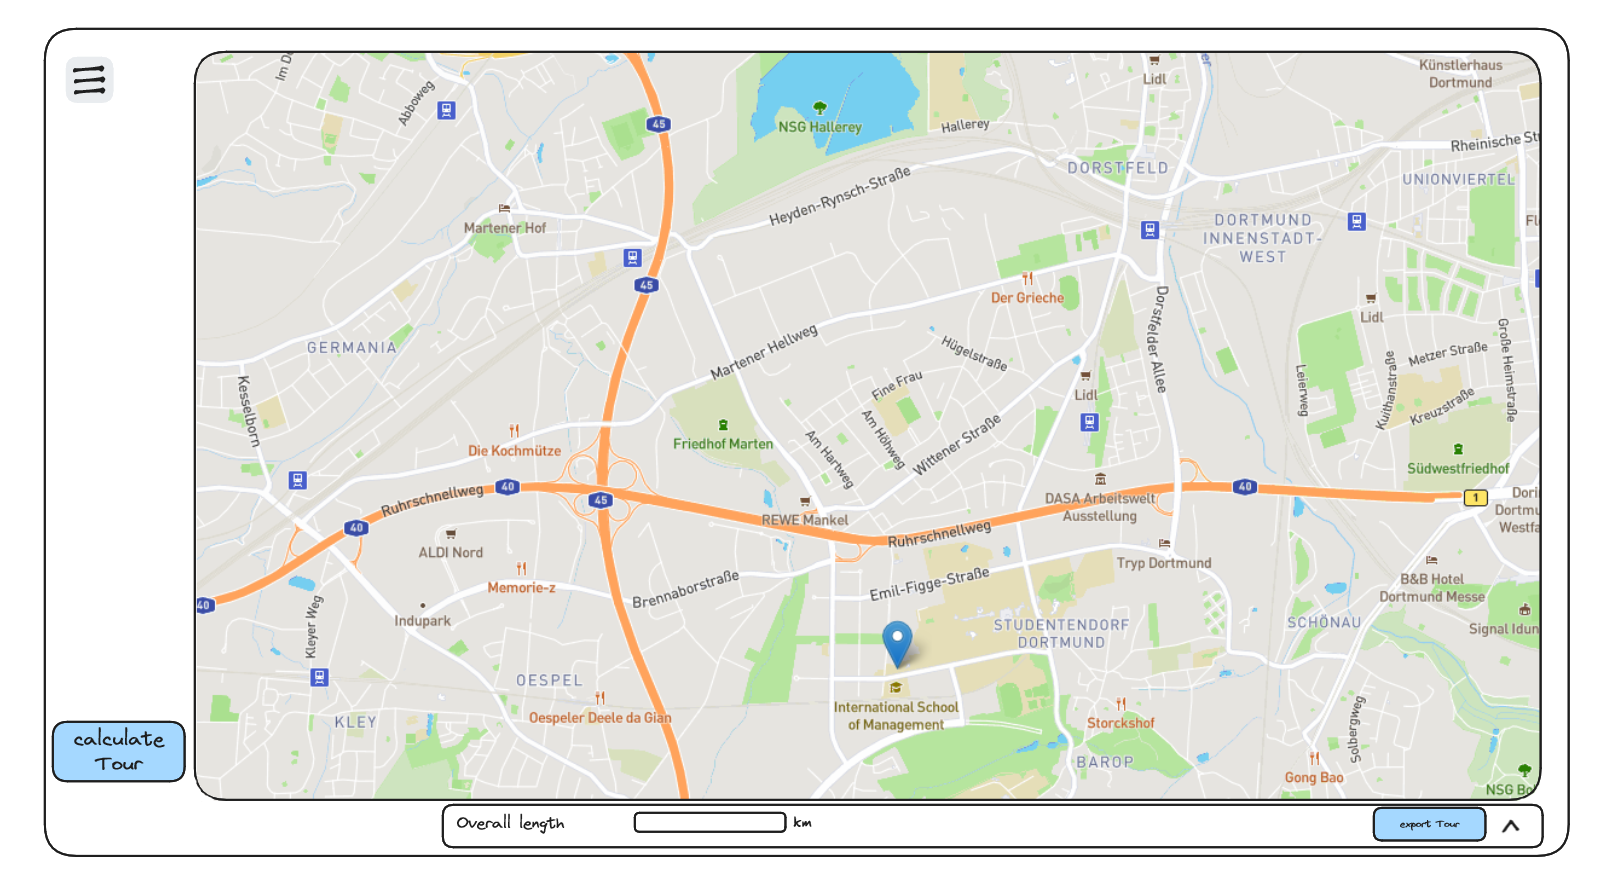
\includegraphics[width=0.9\linewidth]{bilder/Concept burger menu and stats hidden.png}
	\caption{Design concept for the front-end view with all menus folded}
	\label{fig:frontendConceptMenusClosed}
\end{figure}


\begin{figure}[H]
	\begin{subfigure}[t]{0.8\linewidth}
		\centering
		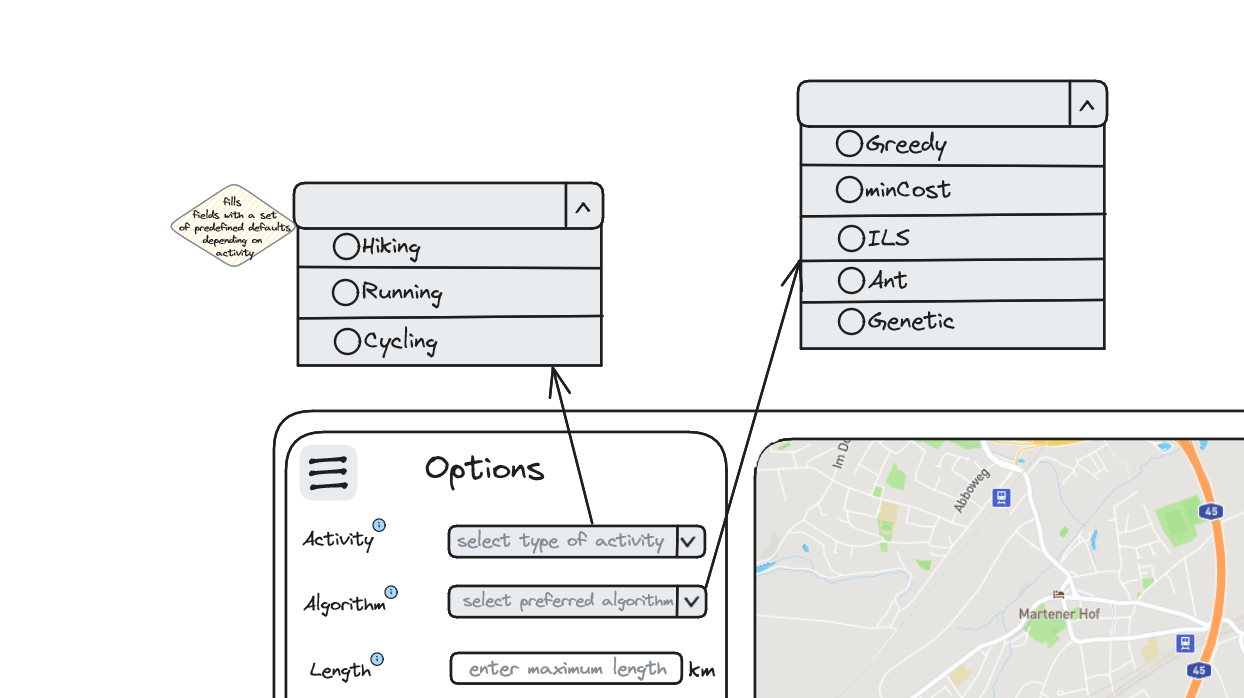
\includegraphics[width=\linewidth]{bilder/Concept closeup activity, algorithm.png}
		\caption{Design concept for the front-end view,closeup of activity and algorithm dropdowns}
		\label{fig:frontendConceptCloseupDropdowns}	
	\end{subfigure}
	\hfill
	\begin{subfigure}[t]{0.8\linewidth}
		\centering
		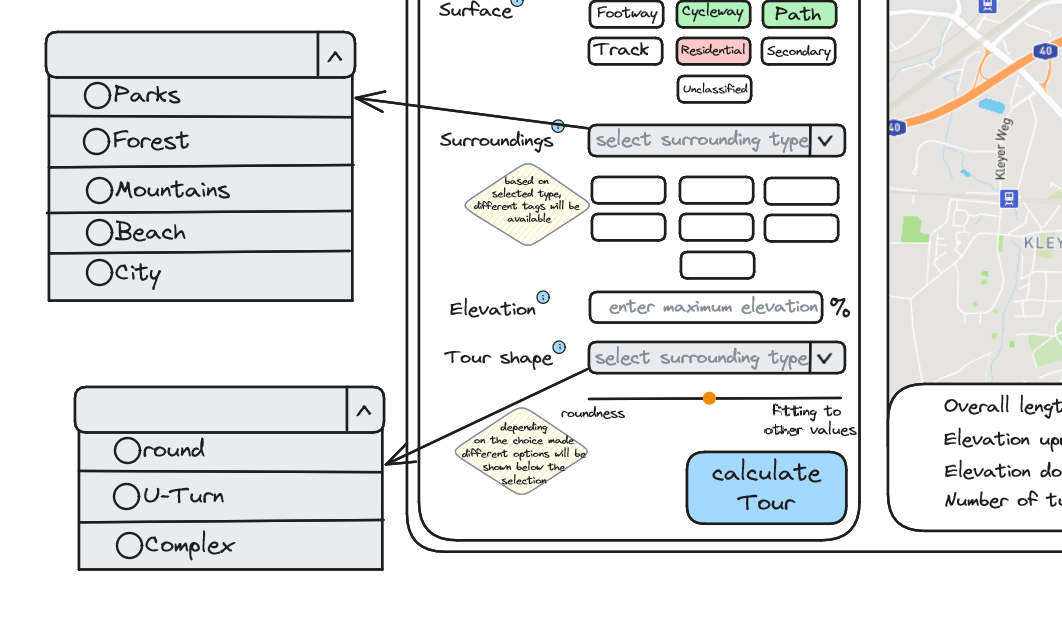
\includegraphics[width=\linewidth]{bilder/Concept closeup surroundings, tour shape.png}
		\caption{Design concept for the front-end view,closeup of a surrounding and Tour shape}
		\label{fig:frontendConceptCloseupButtons}		
	\end{subfigure}
	\caption{Closeups of the side menu design concept}
	\label{fig:frontendSideMenuCloseups}
\end{figure}



\begin{figure}[H]
	\centering
	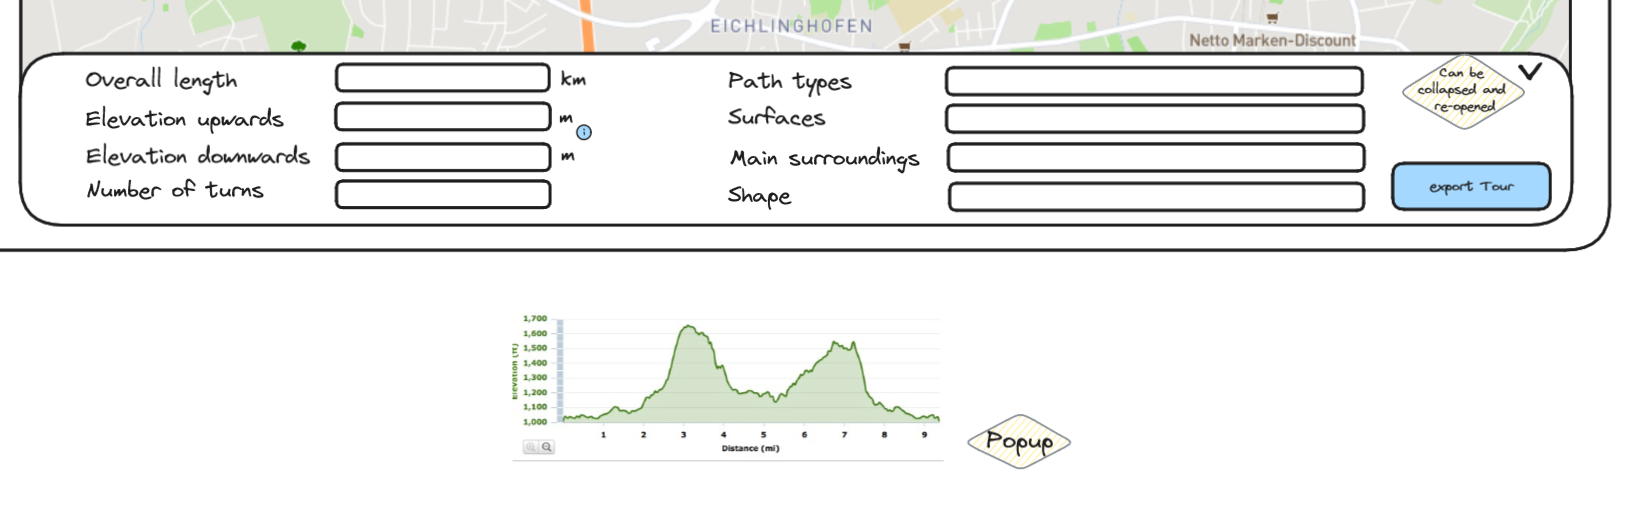
\includegraphics[width=0.9\linewidth]{bilder/Concept closeup tour stats, elevation profile.png}
	\caption{Design concept for the front-end view, closeup of the results view}
	\label{fig:frontendConceptResultsCloseup}
\end{figure}


\begin{figure}[H]
	\centering
	\includegraphics[width=0.9\linewidth]{bilder/actualFrontendSideMenuActivity.png}
	\caption{The options to choose from when the \textit{Activity} drop down is clicked}
	\label{fig:actualFrontendSideMenuActivity}
\end{figure}



\begin{figure}[H]
	\centering
	\includegraphics[width=0.9\linewidth]{bilder/actualFrontendSideMenuAlgorithm.png}
	\caption{The options to choose from when the \textit{Algorithm} drop down is clicked}
	\label{fig:actualFrontendSideMenuAlgorithm}
\end{figure}


\begin{figure}[H]
	\centering
	\includegraphics[width=0.9\linewidth]{bilder/actualFrontendSideMenuSurroundings.png}
	\caption{The options to choose from when the \textit{Surroundings} drop down is clicked}
	\label{fig:actualFrontendSideMenuSurroundings}
\end{figure}


\begin{figure}[H]
	\centering
	\includegraphics[width=0.9\linewidth]{bilder/actualFrontendSideMenuTourShape.png}
	\caption{The options to choose from when the \textit{Tour Shape} drop down is clicked}
	\label{fig:actualFrontendSideMenuTourShape}
\end{figure}








\begin{figure}[H]
	\centering
	\includesvg[width=0.9\textwidth]{bilder/plots/AntFinal/antColonyCasesAlphaVariedAvg.svg}
	\caption{Ant Colony average quality values over varied $\alpha$, $\beta = 1$}
	\label{fig:antColonyCasesAlphaVariedAvg}
\end{figure}


\begin{figure}[H]
	\centering
	\includesvg[width=0.9\textwidth]{bilder/plots/AntFinal/antColonyCasesBetaVariedAvg.svg}
	\caption{Ant Colony average quality values over varied $\beta$, $\alpha = 1$}
	\label{fig:antColonyCasesBetaVariedAvg}
\end{figure}








\begin{figure}[H]
	\centering
	\begin{subfigure}{0.48\textwidth}
		\includesvg[width=0.9\textwidth]{bilder/plots/AntFinal/antColonyCasesAlphaAndBetaVariedSurfaceAvg.svg}
		\caption{Ant Colony average quality values over varied $\alpha$ and $\beta$ surface plot}
		\label{fig:antColonyCasesAlphaAndBetaVariedSurfaceAvg}
	\end{subfigure}
	\hfill
	\begin{subfigure}{0.48\textwidth}
		\includesvg[width=0.9\textwidth]{bilder/plots/AntFinal/antColonyCasesAlphaAndBetaVariedSurfaceAvgTopDown.svg}
		\caption{Ant Colony average quality values over varied $\alpha$ and $\beta$ surface plot top down view}
		\label{fig:antColonyCasesAlphaAndBetaVariedSurfaceAvgTopDown}
	\end{subfigure}
	\caption{Plot of varied $\alpha$ and $\beta$ in different views}
	\label{fig:antColonyCasesAlphaAndBetaVariedAvgAll}
\end{figure}




\begin{figure}[H]
	\centering
	\includesvg[width=0.9\textwidth]{bilder/plots/AntFinal/antColonyCasesNumAnts.svg}
	\caption{Ant Colony average quality values over number ants}
	\label{fig:AntColonyQualityAntsAll}
\end{figure}



\begin{figure}[H]
	\centering
	\includesvg[width=0.9\textwidth]{bilder/plots/AntFinal/antColonyCasesNumAntsAvg.svg}
	\caption{Ant Colony average quality values over number ants}
	\label{fig:AntColonyQualityAntsAvg}
\end{figure}





\begin{figure}[H]
	\centering
	\includesvg[width=0.9\textwidth]{bilder/plots/AntFinal/antColonyCasesCoveredAreaAvg.svg}
	\caption{Ant Colony average covered area values over covered area importance}
	\label{fig:AntColonyAreaAvg}
\end{figure}



\begin{figure}[H]
	\centering
	\includesvg[width=0.9\textwidth]{bilder/plots/AntFinal/antColonyCasesCoveredAreaQualityAvg.svg}
	\caption{Ant Colony average quality values over covered area importance}
	\label{fig:AntColonyAreaQualityAvg}
\end{figure}






\begin{figure}[H]
	\centering
	\includesvg[width=0.9\textwidth]{bilder/plots/AntFinal/antColonyCasesElevationAvg.svg}
	\caption{Ant Colony average elevation values over elevation importance}
	\label{fig:AntColonyElevationAvg}
\end{figure}




\begin{figure}[H]
	\centering
	\includesvg[width=0.9\textwidth]{bilder/plots/AntFinal/antColonyCasesElevationQualityAvg.svg}
	\caption{Ant Colony average quality values over elevation importance}
	\label{fig:AntColonyQualityElevationAvg}
\end{figure}







\begin{figure}[H]
	\centering
	\includesvg[width=0.9\textwidth]{bilder/plots/AntFinal/antColonyCasesProfitAvg.svg}
	\caption{Ant Colony average profit values over profit importance}
	\label{fig:AntColonyProfitAvg}
\end{figure}



\begin{figure}[H]
	\centering
	\includesvg[width=0.9\textwidth]{bilder/plots/AntFinal/antColonyCasesProfitQualityAvg.svg}
	\caption{Ant Colony average quality values over profit importance}
	\label{fig:AntColonyQualityProfitAvg}
\end{figure}






%
%
%\begin{figure}[H]
%	\centering
%	\begin{subfigure}{0.55\textwidth}
%		\includegraphics[width=0.9\linewidth]{bilder/add_move_remove/\texttt{Waypoint},shortest_path&neighbors-move}
%		\caption{Shows the same tour as in \ref{fig:shortestPathAndneighbors} for the \textit{move} operation. 
%			The path fragments to the neighbors that will be changed are highlighted in blue and crossed out. The new path fragments to be added through the moving operation are the green lines. The dotted arrow visualizes the move operation.}
%		\label{fig:shortestPahtAndMove}
%	\end{subfigure}
%	\begin{subfigure}{0.48\textwidth}
%		\includegraphics[width=0.9\linewidth]{bilder/add_move_remove/\texttt{Waypoint},shortest_path&neighbors-changed_after_move}
%		\caption{Shows the same tour as in \ref{fig:shortestPahtAndMove} after the \textit{move} operation.}
%		\label{fig:shortestPathAndMoveDone}
%	\end{subfigure}\hfill
%	\begin{subfigure}{0.5\textwidth}
%	\includegraphics[width=0.9\linewidth]{bilder/add_move_remove/\texttt{Waypoint},shortest_path&neighbors-changed_after_remove}
%	\caption{Shows the same tour as in \ref{fig:shortestPathAndneighbors} after the \textit{remove} operation. The new path fragments to be added through the removing operation are the green lines.}
%	\label{fig:shortestPahtAndRemoveDone}
%	\end{subfigure}
%	
%	\begin{subfigure}{0.45\textwidth}
%	\includegraphics[width=0.9\linewidth]{bilder/add_move_remove/\texttt{Waypoint},shortest_path&neighbors-add}
%	\caption{Shows a tour (black) that is separated in 10 \texttt{Waypoints} (red),a new random \texttt{Waypoint} (green),the closes tour \texttt{Waypoint} and the respective closest of the neighbors (at the end of the blue line fragment). 
%		The path fragment to the neighbor that will be changed is highlighted in blue and crossed out.}
%	\label{fig:shortestPathAndAdd}
%	\end{subfigure}\hfill
%	\begin{subfigure}{0.45\textwidth}
%	\includegraphics[width=0.9\linewidth]{bilder/add_move_remove/\texttt{Waypoint},shortest_path&neighbors-changed_after_add}
%	\caption{Shows the same tour as in \ref{fig:shortestPathAndAdd} after the \textit{add} operation. The new path fragments to be added through the removing operation are the green lines.\textcolor{white}{a\\a\\a\\a}}
%	\label{fig:shortestPathAndAddDone}
%	\end{subfigure}
%	\caption{Visualizations of the add,move and remove operations.}
%	\label{fig:addMoveRemove}
%\end{figure}





\begin{figure}[H]
	\centering
	\includesvg[width=0.9\textwidth]{bilder/plots/SAFinal/SACasesTempFctionTimeMed.svg}
	\caption{Simulated Annealing median time values over runs}
	\label{fig:SATimeOverRuns}
\end{figure}

\begin{figure}[H]
	\centering
	\includesvg[width=0.9\textwidth]{bilder/plots/SAFinal/GenerateTestingValuesSARepititionsMed.svg}
	\caption{Simulated Annealing median quality values over repetitions}
	\label{fig:SAQualityRepititions}
\end{figure}





\begin{figure}[H]
	\centering
	\includesvg[width=0.9\textwidth]{bilder/plots/SAFinal/SACasesNumberRunsCoveredAreaAvg.svg}
	\caption{Simulated Annealing average covered area values over covered area importance}
	\label{fig:SAAreaAvg}
\end{figure}

\begin{figure}[H]
	\centering
	\includesvg[width=0.9\textwidth]{bilder/plots/SAFinal/SACasesNumberRunsCoveredAreaQualityAvg.svg}
	\caption{Simulated Annealing average quality values over covered area importance}
	\label{fig:SAAreaQualityAvg}
\end{figure}




\begin{figure}[H]
	\centering
	\includesvg[width=0.9\textwidth]{bilder/plots/SAFinal/SACasesNumberRunsElevationAvg.svg}
	\caption{Simulated Annealing average elevation values over elevation importance}
	\label{fig:SAElevationAvg}
\end{figure}



\begin{figure}[H]
	\centering
	\includesvg[width=0.9\textwidth]{bilder/plots/SAFinal/SACasesNumberRunsElevationQualityAvg.svg}
	\caption{Simulated Annealing average quality values over elevation importance}
	\label{fig:SAQualityElevationAvg}
\end{figure}



\begin{figure}[H]
	\centering
	\includesvg[width=0.9\textwidth]{bilder/plots/SAFinal/SACasesNumberRunsProfitAvg.svg}
	\caption{Simulated Annealing average edge profit values over edge profit importance}
	\label{fig:SAProfitAvg}
\end{figure}


\begin{figure}[H]
	\centering
	\includesvg[width=0.9\textwidth]{bilder/plots/SAFinal/SACasesNumberRunsProfitQualityAvg.svg}
	\caption{Simulated Annealing average quality values over edge profit importance}
	\label{fig:SAQualityProfitAvg}
\end{figure}






\begin{figure}[H]
	\centering
	\includesvg[width=0.9\textwidth]{bilder/plots/All/AllCasesGreedyMinCostTimeQualityMed.svg}
	\caption{Greedy and MinCosts median quality values over time}
	\label{fig:AllGreedyMinCost}
\end{figure}



\begin{figure}[H]
	\centering
	\includesvg[width=0.9\textwidth]{bilder/plots/All/AllCasesTimeQualityAvg.svg}
	\caption{All implemented algorithms' average quality values over time}
	\label{fig:AllAverage}
\end{figure}



\begin{figure}[H]
	\centering
	\includesvg[width=0.9\textwidth]{bilder/plots/All/AllCasesSATimeQualityAvg.svg}
	\caption{All SA variants' average quality values over time}
	\label{fig:AllSAAverage}
\end{figure}



















\chapter{Additional Pseudocode}

\begin{breakablealgorithm}
	%\begin{algorithm}[ht]
	\caption{Ant Colony}
	\label{alg:AntColony}
	\begin{algorithmic}[1]
		\STATE t $\gets$ 0, NC $\gets$ 0
		\STATE set for all edges(i,j) initial $\tau_{ij}(t) \gets c$ (trail intensiy),$\Delta \tau_{ij} \gets$ 0 
		\STATE Place all m ants on n nodes
		\STATE s (\texttt{tabuList} index) $\gets$ 1
		\FOR{k = 1 to m }
		\STATE add town of m to \texttt{tabuList}
		\WHILE{tabuList not full}
		\STATE s $\gets$ s+1
		\FOR{k = 1 to m}
		\STATE choose nest town to move to with probability $p_{ij}^k(t)$
		\STATE move k-th ant to j
		\STATE add town j to \texttt{tabuList}
		\ENDFOR
		\ENDWHILE
		\FOR{k = 1 to m }
		\STATE move k-th ant back to \texttt{tabuList}(1)
		\STATE calculate length $L_k$ of k's tour
		\STATE Update shortest tour
		\FOR{edge(i,j) in allEdges}
		\FOR{k = 1 to m}
		\STATE $\Delta\tau_{ij}^k = \begin{cases}
			\frac{Q}{L_k}\\
			0
		\end{cases}$
		\STATE $\Delta\tau_{ij} = \Delta\tau_{ij} + \Delta\tau_{ij}^k$
		\ENDFOR
		\ENDFOR
		\ENDFOR
		\FOR{edge(i,j) in allEdges}
		\STATE $\tau_{ij}(t+n)=\rho \cdot \tau_{ij}(t) + \Delta\tau_{ij}$
		\ENDFOR
		\STATE t $\gets$ t+1,NC $\gets$ NC+1
		\FOR{edge(i,j) in allEdges}
		\STATE reset $\Delta\tau_{ij}(t) \gets 0$
		\ENDFOR
		\IF{$NC < NC_{MAX}$ and not stagnating}
		\STATE empty \texttt{tabuList}
		\ELSE
		\STATE return shortest tour
		\ENDIF
		\ENDFOR
	\end{algorithmic}	
	%\end{algorithm}
\end{breakablealgorithm}



\begin{breakablealgorithm}
	\caption{High level Simulated Annealing}
	\label{alg:SApseudocode}
	\begin{algorithmic}[1]
		\STATE i := Select init roundtrip
		\STATE t := Select init temperature 
		\FOR{$i=0$ to numberRepitions}
		\FOR{$i=0$ to numberRuns per temperature}
		\STATE j := Generate neighborhood roundtrip
		\STATE Calculate difference in quality d := f(j)-f(i)
		\IF {d $\geq$ 0}
		\STATE use neighboring solution as current best i $\gets$ j
		\ELSE 
		\STATE random $\gets$ generate random(0,1)
		\IF {random < exp(d/t)} 
		\STATE use neighboring solution as current best i $\gets$ j
		\ENDIF
		\ENDIF
		\ENDFOR
		\STATE update temperature t $\gets$ T(t)
		\ENDFOR
	\end{algorithmic}
\end{breakablealgorithm}




\begin{breakablealgorithm}
	\caption{Simulated Annealing}
	\label{alg:SAImplementation}
	\begin{algorithmic}[1]
		\STATE build \texttt{Waypoint} list (starting point only)
		\STATE (optional; for weighted selection of points) calculateDistances
		\STATE calculate probability distribution
		\STATE t := Select init temperature
		\FOR{$i=0$ to numberRepitions}
		\FOR{$i=0$ to numberRuns per temperature}
		\STATE j := Generate neighborhood roundtrip
		\STATE Calculate difference in quality d := f(j)-f(i)
		\IF {d $\geq$ 0}
		\STATE use neighboring solution as current best i $\gets$ j
		\ELSE 
		\STATE random $\gets$ generate random(0,1)
		\IF {random < exp(d/t)} 
		\STATE use neighboring solution as current best i $\gets$ j
		\ENDIF
		\ENDIF
		\ENDFOR
		\STATE update temperature t $\gets$ T(t)
		\ENDFOR
	\end{algorithmic}
\end{breakablealgorithm}



\begin{breakablealgorithm}
	\caption{Add \texttt{Waypoint}}
	\label{alg:SAGenerateNeigborhoodAdd}
	\begin{algorithmic}[1]
		\STATE calculate shortest path between closest \texttt{Waypoint} (a) and new point (n)
		\STATE calculate shortest path between new point and closer one of the neighbors of closest \texttt{Waypoint} (b)
		\STATE update path from closest \texttt{Waypoint} a
		\STATE add new point n into \texttt{Waypoint} list
		\STATE update path from new point n to b
		\STATE update full tour to include path part a-n-b
	\end{algorithmic}
\end{breakablealgorithm}

\begin{breakablealgorithm}
	\caption{Move closest \texttt{Waypoint}}
	\label{alg:SAGenerateNeigborhoodMove}
	\begin{algorithmic}[1]
		\STATE calculate shortest path between predecessor of closest \texttt{Waypoint} (a) and new point (n)
		\STATE calculate shortest path between new point and successor of closest \texttt{Waypoint} (b)
		\STATE update path from successor of closest \texttt{Waypoint} a
		\STATE update closest \texttt{Waypoint} to be the new point n in \texttt{Waypoint} list
		\STATE update path from new point n to b
		\STATE update full tour to include path part a-n-b
	\end{algorithmic}
\end{breakablealgorithm}

\begin{breakablealgorithm}
	\caption{Remove closest \texttt{Waypoint}}
	\label{alg:SAGenerateNeigborhoodRemove}
	\begin{algorithmic}[1]
		\STATE calculate shortest path between predecessor of closest \texttt{Waypoint} (a) and successor of closest \texttt{Waypoint} (b)
		\STATE update path from successor of closest \texttt{Waypoint} a
		\STATE remove closest \texttt{Waypoint} from \texttt{Waypoint} list
		\STATE update full tour to only include path part a-b
	\end{algorithmic}
\end{breakablealgorithm}


% Literaturverzeichnis
%\bibliographystyle{gerplain}
%\bibliography{literatur/LS11Buchin.bib}
\printbibliography
\addcontentsline{toc}{chapter}{\bibname}


% Abbildungsverzeichnis
\listoffigures
\addcontentsline{toc}{chapter}{List of Figures}
\cleardoublepage
% Algorithmenverzeichnis
\listofalgorithms
\addcontentsline{toc}{chapter}{List of Algorithms}
\cleardoublepage
% Erklaerung
\thispagestyle{myheadings}
\markboth{}{ERKLÄRUNG}
\addcontentsline{toc}{chapter}{Affidavit}
% erklaerung.tex
\cleardoublepage
\normalsize
Hiermit versichere ich, dass ich die vorliegende Arbeit selbstständig verfasst habe und keine anderen als die angegebenen Quellen und Hilfsmittel verwendet sowie Zitate kenntlich gemacht habe.\\\\
Dortmund, den \today \\\\\\\\
Lisa Salewsky
% EOF
\cleardoublepage
\end{document}

